\documentclass[12pt, a4paper]{article}

% --- Essential Packages ---
\usepackage[utf8]{inputenc}
\usepackage{amsmath, amssymb} 
\usepackage{graphicx}         
\usepackage{booktabs}         
\usepackage{pdflscape}

% --- SSRN Document Styling ---
\usepackage[margin=1.25in]{geometry} % Generous margins
\usepackage{setspace}
\onehalfspacing % or \doublespacing for a draft aesthetic

% --- SSRN Citation Style ---
% \usepackage{natbib}
% \bibliographystyle{apalike} 
\usepackage[backend=biber, style=apa, natbib=true]{biblatex}
\addbibresource{references.bib}

% --- Hyperlinks ---
\usepackage[colorlinks=true, linkcolor=blue, citecolor=blue, urlcolor=blue]{hyperref}

% --- Clever References (Load AFTER hyperref) ---
\usepackage{cleveref}

\graphicspath{{images/}}

% --- Custom Commands ---
\usepackage{todonotes}
\newcommand{\extratodo}[1]{\todo[color=blue!30,caption={}]{{\color{blue}#1}}}
\newcommand{\maintodo}[1]{\todo[color=blue!30,inline,caption={}]{{\color{blue}#1}}}

% --- Appendix ---
\usepackage[title,toc]{appendix}

% --- Pretty tables ---
\usepackage{caption}
\captionsetup[table]{labelfont=bf, textfont=bf}
\captionsetup[figure]{labelfont=bf, textfont=bf}
\usepackage{subcaption}
% 1. Create a custom format that says "Panel" before the letter
\DeclareCaptionLabelFormat{panel}{Panel #2}
% 2. Apply it to subtables, make it left-aligned (raggedright), and use a colon
\captionsetup[subtable]{
    labelformat=panel,
    labelsep=colon,
    justification=raggedright,
    singlelinecheck=false, % Forces left-alignment even if the title is short
    font=normalsize % Keeps the font size consistent
}
% 3. Ensure the counter uses uppercase letters (A, B, C)
\renewcommand\thesubtable{\Alph{subtable}}
% 4. Wide tables: sideways
\usepackage{rotating}
% 5. Wrapped tables
\usepackage{tabularx}


% --- Title Page Information ---
\title{\textbf{
    The Geography of Ideology: A Simpson’s Paradox in Stock Market Participation
}}
\author{
    Hyojeong Yoon \\
    \textit{Seoul National University}
}
\date{\today}

\begin{document}

\pagenumbering{roman} % Gives the title page a hidden roman numeral for hyperref

\maketitle

% --- Abstract & Metadata ---
\begin{abstract}
    \noindent Stock market participation is crucial for allocative efficiency across the economy and serves as a primary engine of wealth accumulation for the layperson, yet persistent geographic disparities in participation rates remain a puzzle. This paper uncovers a Simpson’s paradox within participation rate variation across U.S. states. While prior literature suggest individual-level Republican preferences correlate with a higher likelihood of investing, this paper shows that Democratic-leaning states exhibit a significantly higher baseline rate of stock market entry. Furthermore, state-level political environments act as a structural barrier to participation rather than reflecting differences in risk preferences. By proposing potential underlying channels, this study contributes to the intersection of household finance and political economics and opens avenues for further research.

\end{abstract}

\thispagestyle{empty} % Removes the page number from the title page
\newpage
\pagenumbering{arabic} 

% --- Chapters ---
% !TEX root = ../main.tex

\section{Introduction}
\label{sec:intro}

Historically, standard asset pricing models conclude that any risk-averse person should invest at least a fraction of their savings in the stock market to build wealth and earn the equity premium. Yet, in reality, a large portion of the population completely avoids the stock market. This phenomenon is known as the "stock market participation puzzle". 

Understanding why people choose to or not to invest is critical. Theoretically, stock markets act as a vehicle of wealth allocation across agents and across time, facilitating risk-sharing and consumption smoothing to improve allocative efficiency. It is also closely relevant for the layperson, as investing in the stock market is a primary engine of wealth creation and often a major driver of wealth inequality. 

While researchers have identified individual factors like wealth, financial literacy, and social trust that influence this decision \citep{guiso2008, vanrooij2011, bu2022}, an unresolved phenomenon remains: there are persistent geographic differences in participation across U.S. states that cannot be explained by income alone \citep{chien2017}. \citet{chien2017} show that across different income brackets, Connecticut has the highest stock market participation (SMP) rate while Mississippi has the lowest. That is, there is some "black box" driver of SMP that is related to state of residence, but the specific mechanism is not identified.

The main hypothesis in this paper is that the "black box" of geographic differences in stock market participation is the partisan divide between states The motivation comes from the intersection of two strands of literature: (1) the household finance literature on the determinants of stock market participation, and (2) the political economics literature on how political environments shape economic behavior.

Using household-level data from the Panel Study of Income Dynamics (PSID) and state-level political orientation derived from Federal Election Commission (FEC) campaign contributions, this paper explores how living in a predominantly "red" versus "blue" state affects the likelihood of an individual investing in the market.  The findings reveal a textbook case of Simpson's paradox within U.S. financial behavior. On an individual level, shifting toward a Republican leaning increases a person's likelihood of investing, as documented in prior literature. However, in the aggregate, Democratic-leaning states exhibit a significantly higher baseline rate of stock market participation. Furthermore, this geographic divide strictly influences the extensive margin (whether to enter the stock market or not), rather than the intensive margin (how much to allocate to stocks once entered). This suggests that the state-level political environment acts as a structural barrier or fixed cost to market entry, rather than altering investors' risk preferences.

This paper primarily contributes to three specific strands of literature. First, it advances the extensive literature on the stock market participation puzzle and the geographic determinants of portfolio choice. While prior studies have identified that localized factors influence investment decisions, this paper provides a novel, structural explanation for the persistent state-level variations in participation. Crucially, by showing that political geography exclusively affects the extensive margin rather than the intensive margin, it clarifies the mechanism through which geographic environments constrain financial behavior.  

Second, it adds to the growing field of partisan influence on financial decision-making. While existing research demonstrates that individual investors dynamically adjust their risk-taking based on short-term political alignment and partisan optimism, this study establishes that long-term, state-level political environments act as a structural baseline determinant of market entry.  

Finally, this paper provides a distinct empirical contribution by documenting a striking Simpson's paradox within U.S. financial behavior. By disentangling state-level aggregates from individual-level preferences, the findings warn against ecological fallacies in household finance, demonstrating that while individual Republican-leaning preferences may correlate with higher market participation, the overarching structural environment of Democratic-leaning states yields a significantly higher baseline rate of stock ownership.


The remainder of the paper is organized as follows. Section 2 reviews the related literature regarding the stock market participation puzzle and partisan influences on financial decision-making. Section 3 describes the data sources, primarily the Panel Study of Income Dynamics (PSID) and the Federal Election Commission (FEC) campaign finance data, and outlines the methodology for variable construction. Section 4 presents the main empirical results, examining the effect of state-level political environments on both the extensive margin of market participation and the intensive margin of equity shares, alongside several robustness checks. Section 5 reconciles the aggregate state-level findings with established individual-level behavioral theories, formalizing the presence of a Simpson's paradox and addressing the influence of macroeconomic timing. Section 6 discusses potential theoretical channels and structural factors that might drive these observed geographic disparities. Finally, Section 7 concludes.
% !TEX root = ../main.tex

\section{Related Literature}
\label{sec:litreview}

Standard portfolio theory suggests that risk-averse investors should hold some portion of their wealth in a diversified portfolio of equities to earn the equity premium. However, the actual stock market participation (SMP) rate is significantly lower than predicted, a puzzle widely documented in the foundational literature. Subsequent studies have explored various determinants to explain this participation puzzle. \citet{menkhoff2025} provide a comprehensive overview, categorizing the drivers into direct costs such as wealth and income \citep{guiso2008}, knowledge and cognitive abilities \citep{vanrooij2011}, individual trust \citep{guiso2008, bu2022}, and peer effects through sociability and networks \citep{hong2004, brown2008}. 

In this paper, I focus on a yet unexplained pattern: the persistent geographic variation in SMP across U.S. states, which cannot be fully accounted for by differences in income \citep{chien2017}. Prior literature has used state-level variances to isolate driving factors of SMP. \citet{brown2004} find that individuals in states with higher average SMP are more likely to participate themselves, suggesting a community ownership effect. \citet{giannetti2016} use a 2002 corporate fraud scandal to show that corporate fraud revelation leads to lower SMP and decreased stock holdings in all firms, suggesting a local shock to trust in the stock market. Also suggestive of a trust channel, \citet{huang2023} find that states with higher accounting quality, proxied by audit market size, exhibit higher SMP.  

Another crucial driver of stock market participation is the political orientation of the investor. Using Finnish data, \citet{kaustia2011} find that right-leaning individuals are more likely to participate in the stock market. However, when extended to other European countries, \citet{kaustia2023} find that the relationship between right-leaning political orientation and SMP is not consistent, particularly in countries with low regulatory quality. In the United States, research has shown an alignment effect: individuals become more optimistic and perceive markets as less risky when their preferred political party is in power, which consequently boosts their likelihood to invest \citep{bonaparte2017}. Building on this, \citet{meeuwis2022} demonstrate that likely-Republicans increased the equity share of their portfolios relative to Democrats immediately following the 2016 presidential election.  

While \citet{meeuwis2022} focus on the immediate, short-term rebalancing of equity shares within existing brokerage accounts around a specific election event, this paper examines baseline stock market participation rates during normal times. Furthermore, while previous studies have often relied on U.S. data that is fragmented across different time periods for stock market variables versus political indicators, this study employs unified datasets to test the state-level political stance and its dual-channel effect on SMP. 
% !TEX root = ../main.tex

\section{Data and Methodology}
This section describes the data sources, cleaning methods, and variable construction processes. Two primary datasets are utilized: the Panel Study of Income Dynamics (PSID) for household-level stock market participation and the Federal Election Commission (FEC) Campaign Finance data for state-level political orientation. Additional datasets are employed for robustness checks in later sections when necessary (see \Cref{sec:robust_x} and \Cref{sec:robust_y}).

\subsection{Stock Market Participation Data}
\label{sec:data_psid}

For household-level stock market participation, the data is from the Panel Study of Income Dynamics (PSID) \citep{PSID2024}. The PSID provides longitudinal, household-level data detailing state of residence, stock ownership, wealth, and demographic information. The sample period covers 1999 to 2023 at a biennial frequency in odd years, restricted by availability of stock holdings data. 

The dataset features a panel structure constructed at the family level (i = family, t = year). A representative person is interviewed from each family. Income, wealth, and stock market holding (which explicitly excludes retirement accounts but includes mutual funds) are aggregated at the family unit. Demographic characteristics—such as education and gender are extracted for the representative person. 

One limiting characteristic of the PSID is its oversampling of low-income families. However, this bias is not a concern for this analysis. First, the primary focus is on the relationship between political orientation and stock market participation rather than estimating population-level participation rates. For the same reasons, sampling weights are not applied in the regression analyses. Second, the main regressions control for income and wealth at the household level.

For each family-year observation, the following variables are constructed:
\begin{itemize}
    \item \texttt{stockhold}: binary indicator equal to 1 if the family has direct holdings in stocks (including mutual funds with stocks, excluding retirement accounts) and 0 otherwise.
    \item \texttt{finassets}: total financial assets, calculated as the sum of cash, bonds, and stocks.
    \item \texttt{stockshare}: the share of financial assets held in stocks, calculated as the ratio of stock holdings to total financial assets, capped at 1.
    \item \texttt{ln(income)}: natural logarithm of total family income.    
    \item \texttt{ln(wealth)}: natural logarithm of total family wealth.
    \item \texttt{college}: binary indicator equal to 1 if the representative person has a college degree and 0 otherwise.
    \item \texttt{age}: age of the representative person.
    \item \texttt{male}: binary indicator equal to 1 if the representative person is male and 0 otherwise.
\end{itemize}
See \Cref{sec:appendix_psid} for detailed variable construction processes and the specific PSID variable codes used.


\subsection{Political Data}
\label{sec:data_political}

To proxy state-level political orientation, this paper follows \citet{meeuwis2022} and uses the Federal Election Commission (FEC) Campaign Finance data \citep{FEC2024}.

Individual contributions to presidential candidates and political parties are obtained from the FEC campaign finance data. \citet{meeuwis2022} uses the same data to construct zip-code level political orientations and connects them to propreitary brokerage data with zip-code geographic granularity. In this paper, the FEC data is used to construct a state-level political orientation variable, which serves as the main independent variable in the analysis. Specifically, valid contributions made to committees that directly support specific candidates or parties are aggregated at the state-year level. Contributions supporting lost primary candidates or specific issues are excluded. See \Cref{sec:appendix_fecscreen} for a detailed description of the variable construction process. After aggregating, two measures of political orientation are constructed: (1) STDIR(A) from the total amount of contributions and (2) STDIR(N) from the total number of contributions.

$$
STDIR(A)_{s,t} = 2 \times \left( \frac{\text{Total Contribution Amount to Republican Committees}_{s,t}}{\text{Total Contribution Amount}_{s,t}} \right) - 1
$$
$$
STDIR(N)_{s,t} = 2 \times \left( \frac{\text{Total Contribution Number to Republican Committees}_{s,t}}{\text{Total Contribution Number}_{s,t}} \right) - 1
$$

Both measures are normalized to be bounded between -1 and 1, where -1 indicates a fully Democratic-leaning state and 1 indicates a fully Republican-leaning state. Such normalization is motivated for the ease of constructing the alignment variable. Defining FEDIR, the federal political direction variable, as 1 during Republican presidencies and -1 during Democratic presidencies, the state-federal alignment variable (STALG) is constructed as the interaction between the state and federal political directions:
$$
STALG_{s,t} = STDIR_{s,t} \times FEDIR_t
$$
A positive STALG value denotes political alignment between the state and the federal executive branch (Republican-leaning state under a Republican president or Democratic-leaning state under a Democratic president), while a negative value signifies misalignment.

\subsection{Summary Statistics}
\label{sec:summary_stats}

\begin{table}[htbp]
    \caption{Summary Statistics}
    \label{tab:1}

    \begin{minipage}{\textwidth}
        \small This table presents summary statistics for the main variables used in the analysis. The sample is a panel dataset covering families in the PSID dataset during 1999-2023. PSID variables are at the family-year level, while the FEC variables are at the state-year level.
    \end{minipage}

    \vspace{1ex}

    \small 

    {
\def\sym#1{\ifmmode^{#1}\else\(^{#1}\)\fi}
\begin{tabular*}{\textwidth}{l@{\extracolsep{\fill}}*{6}{c}}
\toprule
          &        N&     Mean&       SD&     25th&   Median&     75th\\
\midrule
1(Stockhold)&  111,231&    0.152&    0.359&    0.000&    0.000&    0.000\\
income    &  109,875&70549.153&98293.970&25400.000&49560.000&88500.000\\
wealth    &   86,781&320746.037&1251299.302&15700.000&75300.000&256200.000\\
1(College)&  111,048&    0.300&    0.458&    0.000&    0.000&    1.000\\
Age       &  111,208&   45.706&   16.379&   32.000&   43.000&   57.000\\
1(Male)   &  111,231&    0.685&    0.465&    0.000&    1.000&    1.000\\
STDIR(A)  &  111,231&    0.156&    0.375&   -0.127&    0.241&    0.457\\
STDIR(N)  &  111,231&    0.073&    0.418&   -0.273&    0.151&    0.421\\
FEDIR     &  111,231&   -0.093&    0.996&   -1.000&   -1.000&    1.000\\
STALG(A)  &  111,231&   -0.021&    0.405&   -0.361&   -0.066&    0.310\\
STALG(N)  &  111,231&   -0.037&    0.422&   -0.395&   -0.064&    0.330\\
\bottomrule
\end{tabular*}
}

\end{table}

\Cref{tab:1} presents the summary statistics for the main variables used in the analysis. The sample contains up to $111,231$ observations, though variables such as Income ($N=109,875$) and Wealth ($N=86,781$) exhibit slightly lower counts due to missing data. 

Financially, the stockholding indicator (1(Stockhold)) demonstrates a mean of $0.152$, implying that $15.2\%$ of the individuals in the sample participate in the stock market. This is in line with the commonly cited estimates from the Survey of Consumer Finances (SCF). Excluding retirement accounts, the SCF reports that the percentage of American families with direct stock holdings was 15\% in 2019 and 21\% in 2022 \citep{SCF2023}. Income and Wealth variables show high variation and skewness, which is typical for financial data. Accordingly, these variables are log-transformed in the regression analyses.

The demographic composition of the sample shows an average age of $45.7$ years (Age mean $= 45.706$) and an educational attainment rate where $30.0\%$ of respondents hold a college degree (1(College) mean $= 0.300$). This educational metric is relatively proximate, though slightly lower. The U.S. Census Bureau Educational Attainment statistics show that around half of American adults aged 25 and older have obtained an associate degree or higher \citep{Census2024}. The sample is disproportionately male at $68.5\%$ (1(Male) mean $= 0.685$). This could be a result of male partners being more likely to be the representative person being interviewed, rather than a overrepresentation of men in the PSID sample.

Although the summary averages reveal some deviations from aggregate U.S. population statistics, the exact baseline levels of these variables are not critical to the integrity of this study. The primary objective of the empirical framework is to identify the underlying relationships and marginal effects among these covariates. As long as there is sufficient variation within the sample to capture these dynamics the representativeness of the point estimates remains secondary to the structural relationships being analyzed.

The FEC contribution variables are measured at the state-year level. The state-level political direction (STDIR) captures the political leaning of a state based on Federal Election Commission (FEC) data, bounded between -1 (fully Democratic) and 1 (fully Republican). The direction measures exhibit slight Republican leans, with means of 0.152 and 0.068, respectively. Both measures show substantial variation, as evidenced by their standard deviations ranging from 0.179 to 0.418.

The federal political direction (FEDIR) is an indicator variable that takes a value of 1 during a Republican presidency and -1 during a Democratic presidency. The variable has a mean of -0.093, which simply reflects that within this specific 1999-2023 panel dataset, slightly more family-year observations occurred under Democratic administrations than Republican ones.

Finally, the state-federal alignment variable (STALG) represents the interaction between the state's political leaning and the president's party (STDIR × FEDIR). A positive STALG value denotes political alignment between the state and the federal executive branch (e.g., a Republican-leaning state under a Republican president), while a negative value signifies misalignment. The means for STALG(A) and STALG(N) are -0.022 and -0.039, respectively. These near-zero averages indicate that, across the sample period, respondents' state-level political environments were relatively evenly split between being aligned and misaligned with the party in control of the White House.
% !TEX root = ../main.tex

\section{Results}
\label{sec:results}

\subsection{Baseline Results}
Before moving onto the main analysis, I first present baseline evidence that there are indeed persistent geographic differences in stock market participation (SMP). This step is necessary because \citet{chien2017} utilize a different dataset: state-level aggregates of IRS tax return data, where the state-level SMP rate is calculated as the fraction of tax returns with dividend income out of total tax returns filed.

\Cref{tab:2} presents the baseline results. Columns 1 and 2 are linear probability models (LPM), while columns 3 and 4 are Probit models. The coefficients on the control variables are consistent with established household finance literature: wealth, income, and education all exhibit positive and highly significant effects on the likelihood of participation.Columns 1 and 3 include individual controls and time fixed effects, whereas columns 2 and 4 further include state fixed effects. 

The test statistics and p-values reported are for the joint hypothesis test on the null that all state fixed effects are jointly zero. In both models, the p-value is close to zero, confirming the presence of persistent geographic differences in SMP. Specifically, in column 2 (LPM), the reported state joint statistic of 18.0 is from OLS and represents an F-test. In column 4 (Probit), the joint statistic of 490 is from maximum likelihood estimation with robust standard errors and represents a Wald test that follows a $\chi^2$ distribution. Both tests evaluate the null hypothesis that the state-specific intercepts are simultaneously zero, and both decisively reject it.

Despite confirming the presence of geographic effects, these baseline models suffer from notable limitations regarding statistical and explanatory power. By relying solely on static state fixed effects, the specification functions as a "black box," failing to identify the actual underlying mechanisms. Consequently, the model lacks the explanatory power to detail why these geographic differences exist. This motivates the subsequent analysis stemming from the hypothesis that the "black box" of geographic differences in SMP is captured by state politics. 



\begin{table}[htbp]
\caption{Baseline Results}
\label{tab:2}
\begin{minipage}{\textwidth}
    \small This table presents the baseline linear probability and probit models predicting stock market participation. The dependent variable is a binary indicator equal to one if the individual holds stocks, and zero otherwise. Continuous independent variables ln(Income), ln(Wealth), and Age are standardized to have mean zero and standard deviation one. 1(College) and 1(Male) are binary variables each equal to one if the representative person of the family has a college degree and is male, respectively. Time fixed effects are included. For probit models, the reported values are marginal effects evaluated at the mean of the independent variables. Robust standard errors clustered at the state level are reported in parentheses. *** p $<$ 0.01, ** p $<$ 0.05, * p $<$ 0.1.
\end{minipage}

\small

\vspace{1ex}

{
\def\sym#1{\ifmmode^{#1}\else\(^{#1}\)\fi}
\begin{tabular*}{\textwidth}{l@{\extracolsep{\fill}}*{4}{c}}
\toprule
          &\multicolumn{2}{c}{LPM}              &\multicolumn{2}{c}{Probit}           \\
          &\multicolumn{1}{c}{(1)}&\multicolumn{1}{c}{(2)}&\multicolumn{1}{c}{(3)}&\multicolumn{1}{c}{(4)}\\
          &\multicolumn{1}{c}{stockhold}&\multicolumn{1}{c}{stockhold}&\multicolumn{1}{c}{stockhold}&\multicolumn{1}{c}{stockhold}\\
\midrule
ln(Income)&    0.034\sym{***}&    0.030\sym{***}&    0.032\sym{***}&    0.029\sym{***}\\
          &  (0.002)         &  (0.002)         &  (0.002)         &  (0.002)         \\
\addlinespace
ln(Wealth)&    0.116\sym{***}&    0.115\sym{***}&    0.157\sym{***}&    0.153\sym{***}\\
          &  (0.002)         &  (0.002)         &  (0.002)         &  (0.002)         \\
\addlinespace
1(College)&    0.146\sym{***}&    0.143\sym{***}&    0.110\sym{***}&    0.108\sym{***}\\
          &  (0.003)         &  (0.003)         &  (0.003)         &  (0.003)         \\
\addlinespace
Age       &    0.009\sym{***}&    0.008\sym{***}&   -0.006\sym{***}&   -0.006\sym{***}\\
          &  (0.001)         &  (0.001)         &  (0.001)         &  (0.001)         \\
\addlinespace
1(Male)   &   -0.004         &   -0.004         &   -0.009\sym{***}&   -0.010\sym{***}\\
          &  (0.003)         &  (0.003)         &  (0.003)         &  (0.003)         \\
\midrule
\(N\)     &    86066         &    86066         &    86066         &    86066         \\
State FE  &       No         &      Yes         &       No         &      Yes         \\
Year FE   &      Yes         &      Yes         &      Yes         &      Yes         \\
State Joint Stat.&        -         &  1.8e+01         &        -         &  4.9e+02         \\
State P-Value&        -         &  6.e-153         &        -         &  2.0e-73         \\
R-sq      &    0.206         &    0.212         &    0.262         &    0.268         \\
\bottomrule
\end{tabular*}
}


\end{table}


\subsection{Stock Market Participation}
\label{sec:main_smp}

% --- Table 3 ---
% --- PAGE 1: PANEL A ---
\begin{table}[htbp]
    \centering
    \caption{Stock Market Participation and State Politics}
    \label{tab:3}

    \begin{minipage}{\textwidth}
    \small This table presents regression results for the determinants of stock market participation. Panel A uses linear probability models (LPM), while Panel B uses Probit models. The dependent variable is a binary indicator equal to one if the individual holds stocks, and zero otherwise. The independent variables STDIR(A) and STDIR(N) are state-level continuous measures of political direction, ranging from 1 (all Republican contributions) to -1 (all Democratic contributions). FEDIR is a binary time series variable equal to one if the president is a Republican and -1 if the president is a Democrat. STALG(A) and STALG(N) are the interaction terms between the state political direction variables and FEDIR Continuous control variables ln(Income), ln(Wealth), and Age are standardized to have mean zero and standard deviation one. 1(College) and 1(Male) are binary control variables each equal to one if the representative person of the family has a college degree and is male, respectively. Time fixed effects are included. For probit models, the reported values are marginal effects evaluated at the mean of the explanatory variables. Robust standard errors clustered at the state level are reported in parentheses. *** p $<$ 0.01, ** p $<$ 0.05, * p $<$ 0.1.
    \end{minipage}

    \small 

    \vspace{1ex}
    
    \begin{subtable}{\textwidth}
        \caption{Linear Probability Model (LPM)}
        \label{tab:3a}
        {
\def\sym#1{\ifmmode^{#1}\else\(^{#1}\)\fi}
\begin{tabular}{l*{6}{c}}
\toprule
                    &\multicolumn{1}{c}{(1)}&\multicolumn{1}{c}{(2)}&\multicolumn{1}{c}{(3)}&\multicolumn{1}{c}{(4)}&\multicolumn{1}{c}{(5)}&\multicolumn{1}{c}{(6)}\\
                    &\multicolumn{1}{c}{stockhold}&\multicolumn{1}{c}{stockhold}&\multicolumn{1}{c}{stockhold}&\multicolumn{1}{c}{stockhold}&\multicolumn{1}{c}{stockhold}&\multicolumn{1}{c}{stockhold}\\
\midrule
ln(Income)          &       0.033\sym{***}&       0.032\sym{***}&       0.034\sym{***}&       0.034\sym{***}&       0.033\sym{***}&       0.032\sym{***}\\
                    &     (0.003)         &     (0.003)         &     (0.003)         &     (0.003)         &     (0.003)         &     (0.003)         \\
\addlinespace
ln(Wealth)          &       0.116\sym{***}&       0.116\sym{***}&       0.116\sym{***}&       0.116\sym{***}&       0.116\sym{***}&       0.116\sym{***}\\
                    &     (0.005)         &     (0.005)         &     (0.005)         &     (0.005)         &     (0.005)         &     (0.005)         \\
\addlinespace
1(College)          &       0.145\sym{***}&       0.145\sym{***}&       0.146\sym{***}&       0.146\sym{***}&       0.145\sym{***}&       0.145\sym{***}\\
                    &     (0.007)         &     (0.007)         &     (0.007)         &     (0.007)         &     (0.007)         &     (0.007)         \\
\addlinespace
Age                 &       0.009\sym{***}&       0.008\sym{***}&       0.009\sym{***}&       0.009\sym{***}&       0.008\sym{***}&       0.008\sym{***}\\
                    &     (0.002)         &     (0.003)         &     (0.002)         &     (0.002)         &     (0.003)         &     (0.003)         \\
\addlinespace
1(Male)             &      -0.004         &      -0.004         &      -0.004         &      -0.004         &      -0.004         &      -0.004         \\
                    &     (0.006)         &     (0.006)         &     (0.006)         &     (0.006)         &     (0.006)         &     (0.006)         \\
\addlinespace
STDIR(A)            &      -0.042\sym{***}&                     &                     &                     &      -0.043\sym{***}&                     \\
                    &     (0.012)         &                     &                     &                     &     (0.012)         &                     \\
\addlinespace
STDIR(N)            &                     &      -0.066\sym{***}&                     &                     &                     &      -0.067\sym{***}\\
                    &                     &     (0.015)         &                     &                     &                     &     (0.016)         \\
\addlinespace
STALG(A)            &                     &                     &       0.003         &                     &      -0.003         &                     \\
                    &                     &                     &     (0.004)         &                     &     (0.004)         &                     \\
\addlinespace
STALG(N)            &                     &                     &                     &       0.009\sym{*}  &                     &      -0.005         \\
                    &                     &                     &                     &     (0.005)         &                     &     (0.005)         \\
\addlinespace
FEDIR               &                     &                     &                     &                     &      -0.094\sym{***}&      -0.119\sym{***}\\
                    &                     &                     &                     &                     &     (0.005)         &     (0.008)         \\
\midrule
Obs.                &      86,066         &      86,066         &      86,066         &      86,066         &      86,066         &      86,066         \\
R-sq                &       0.207         &       0.207         &       0.206         &       0.206         &       0.207         &       0.207         \\
\bottomrule
\end{tabular}
}

    \end{subtable}
\end{table}

% --- PAGE 2: PANEL B ---
\begin{table}[htbp]
    \ContinuedFloat
    \centering

    \caption[]{Stock Market Participation and State Politics (Cont.)}
    
    \small
    
    \begin{subtable}{\textwidth}
        \caption{Probit Model}
        \label{tab:3b}
        {
\def\sym#1{\ifmmode^{#1}\else\(^{#1}\)\fi}
\begin{tabular}{l*{6}{c}}
\toprule
                    &\multicolumn{1}{c}{(1)}&\multicolumn{1}{c}{(2)}&\multicolumn{1}{c}{(3)}&\multicolumn{1}{c}{(4)}&\multicolumn{1}{c}{(5)}&\multicolumn{1}{c}{(6)}\\
                    &\multicolumn{1}{c}{stockhold}&\multicolumn{1}{c}{stockhold}&\multicolumn{1}{c}{stockhold}&\multicolumn{1}{c}{stockhold}&\multicolumn{1}{c}{stockhold}&\multicolumn{1}{c}{stockhold}\\
\midrule
ln(Income)          &       0.031\sym{***}&       0.031\sym{***}&       0.032\sym{***}&       0.032\sym{***}&       0.031\sym{***}&       0.031\sym{***}\\
                    &     (0.003)         &     (0.003)         &     (0.003)         &     (0.003)         &     (0.003)         &     (0.003)         \\
\addlinespace
ln(Wealth)          &       0.156\sym{***}&       0.155\sym{***}&       0.157\sym{***}&       0.157\sym{***}&       0.156\sym{***}&       0.155\sym{***}\\
                    &     (0.005)         &     (0.005)         &     (0.004)         &     (0.004)         &     (0.005)         &     (0.005)         \\
\addlinespace
college=1           &       0.110\sym{***}&       0.110\sym{***}&       0.110\sym{***}&       0.110\sym{***}&       0.110\sym{***}&       0.110\sym{***}\\
                    &     (0.006)         &     (0.005)         &     (0.006)         &     (0.006)         &     (0.006)         &     (0.005)         \\
\addlinespace
Age                 &      -0.005\sym{**} &      -0.005\sym{**} &      -0.006\sym{**} &      -0.006\sym{**} &      -0.005\sym{**} &      -0.005\sym{**} \\
                    &     (0.002)         &     (0.002)         &     (0.002)         &     (0.002)         &     (0.002)         &     (0.002)         \\
\addlinespace
male=1              &      -0.009         &      -0.009         &      -0.009         &      -0.009         &      -0.009         &      -0.009         \\
                    &     (0.006)         &     (0.006)         &     (0.006)         &     (0.006)         &     (0.006)         &     (0.006)         \\
\addlinespace
STDIR(A)            &      -0.027\sym{**} &                     &                     &                     &      -0.027\sym{**} &                     \\
                    &     (0.012)         &                     &                     &                     &     (0.012)         &                     \\
\addlinespace
STDIR(N)            &                     &      -0.044\sym{***}&                     &                     &                     &      -0.044\sym{**} \\
                    &                     &     (0.017)         &                     &                     &                     &     (0.017)         \\
\addlinespace
STALG(A)            &                     &                     &       0.004         &                     &      -0.001         &                     \\
                    &                     &                     &     (0.004)         &                     &     (0.003)         &                     \\
\addlinespace
STALG(N)            &                     &                     &                     &       0.011\sym{**} &                     &       0.004         \\
                    &                     &                     &                     &     (0.005)         &                     &     (0.005)         \\
\addlinespace
FEDIR               &                     &                     &                     &                     &      -0.097\sym{***}&      -0.112\sym{***}\\
                    &                     &                     &                     &                     &     (0.004)         &     (0.009)         \\
\midrule
Obs.                &      86,066         &      86,066         &      86,066         &      86,066         &      86,066         &      86,066         \\
R-sq                &       0.262         &       0.263         &       0.262         &       0.262         &       0.262         &       0.263         \\
\bottomrule
\end{tabular}
}

    \end{subtable}
    
    \vspace{1ex}

\end{table}


\Cref{tab:3} presents the main results for the determinants of stock market participation, utilizing Linear Probability Models (LPM) in Panel A and Probit models in Panel B.

Before evaluating the political variables, it is worth noting that the baseline household finance controls behave consistently with established theory across all specifications. Because the continuous variables are standardized, their coefficients represent the effect of a one standard deviation increase. A one standard deviation increase in log wealth massively boosts the probability of holding stocks by 11.6 to 15.7 percentage points, while a similar increase in log income raises the probability by roughly 3.1 to 3.4 percentage points. Educational attainment is also a powerful driver. Individuals with a college degree are 11.0 to 14.6 percentage points more likely to participate in the market.Interestingly, the coefficient for the male indicator is statistically insignificant across all columns in both panels. While unconditional demographic data sometimes highlights a gender gap in investing \citep{almenberg2015}, this insignificance is both acceptable and expected in this framework. As noted in \Cref{sec:summary_stats}, because the PSID operates at the family-year level, the gender of the representative person often reflects survey response dynamics rather than a strict measure of individual gender behavior. By controlling for income, wealth, and education, the model absorbs the underlying disparities that typically drive gender differences in financial participation. Additionally, Age exhibits a statistically significant but marginal effect, serving more as a necessary life-cycle control than a primary driver.

Turning to the primary variables of interest, Columns 1 and 2 show that the absolute state political direction variables STDIR(A) and STDIR(N) have significant and negative coefficients. Because STDIR ranges from 1 (all Republican contributions) to -1 (all Democratic contributions), this negative coefficient indicates that, after controlling for individual characteristics and time fixed effects, individuals living in states with more Democratic contributions are more likely to hold stocks. This macro-level result seems to contradict the individual-level findings in prior literature demonstrating that right-leaning individuals are more likely to participate in the stock market \citep{kaustia2011, ke2024}. However, as will be elaborated in \Cref{sec:reconc}, this divergence is a manifestation of Simpson's paradox. The state-level aggregation masks the true individual-level behaviors, meaning these findings do not actually contradict established individual-level theories.

Columns 3 and 4 introduce the state political alignment, or the interaction terms between state political direction and federal government direction (STALG(A) and STALG(N)). As seen in Column 4 of both panels, the STALG(N) specification yields a positive and statistically significant coefficient. At first glance, this positive significance might seem to support the partisan alignment effect documented in prior literature, which suggests individuals are more likely to invest when their political environments or personal preferences align with the party in power \citep{bonaparte2017, meeuwis2022}.

However, Columns 5 and 6 reveal that this interpretation is premature. By including the baseline federal direction variable (FEDIR), the model controls for the time-series effect of the presidential party applied across all states. Once FEDIR is introduced, the coefficients on the alignment variables lose significance. This indicates that the initial significance observed in Column 4 was merely a confounded effect driven by the omission of the federal-level baseline.

Instead, the dominant effect emerges directly from the FEDIR variable, which exhibits strong, negative, and highly significant coefficients across both models. Because FEDIR equals 1 during Republican presidencies, this implies that aggregate stock market participation within the sample is systematically lower under Republican administrations, holding all else constant. As will be in seen in \Cref{sec:reconc_alg}, this is likely a consequence of sample-specific coincidences between the timing of presidential terms and macroeconomic conditions that broadly suppressed stock market participation.

\subsection{Equity Share}
\label{sec:main_eqshare}

% --- PAGE 1: PANEL A ---
\begin{table}[htbp]
    \centering
    \caption{Equity Share and State Politics}
    \label{tab:4}

    \begin{minipage}{\textwidth}
    \small This table presents regression results for the determinants of equity share among stock market participants. Panel A uses ordinary least squares (OLS), while Panel B uses fractional Probit models. The dependent variable is the proportion of financial assets held in stocks, from 0 to 1. The independent variables STDIR(A) and STDIR(N) are state-level continuous measures of political direction, ranging from 1 (all Republican contributions) to -1 (all Democratic contributions). FEDIR is a binary time series variable equal to one if the president is a Republican and -1 if the president is a Democrat. STALG(A) and STALG(N) are the interaction terms between the state political direction variables and FEDIR Continuous control variables ln(Income), ln(Wealth), and Age are standardized to have mean zero and standard deviation one. 1(College) and 1(Male) are binary control variables each equal to one if the representative person of the family has a college degree and is male, respectively. Time fixed effects are included. For probit models, the reported values are marginal effects evaluated at the mean of the explanatory variables. Robust standard errors clustered at the state level are reported in parentheses. *** p $<$ 0.01, ** p $<$ 0.05, * p $<$ 0.1.
    \end{minipage}

    \small 

    \vspace{1ex}
    
    \begin{subtable}{\textwidth}
        \caption{Ordinary Least Squares (OLS)}
        \label{tab:4a}
        \input{tables/tb4A.tex}
    \end{subtable}
\end{table}

% --- PAGE 2: PANEL B ---
\begin{table}[htbp]
    \ContinuedFloat
    \centering

    \caption[]{Equity Share and State Politics (Cont.)}
    
    \small
    
    \begin{subtable}{\textwidth}
        \caption{Fractional Probit Model}
        \label{tab:4b}
        {
\def\sym#1{\ifmmode^{#1}\else\(^{#1}\)\fi}
\begin{tabular}{l*{6}{c}}
\toprule
                    &\multicolumn{1}{c}{(1)}&\multicolumn{1}{c}{(2)}&\multicolumn{1}{c}{(3)}&\multicolumn{1}{c}{(4)}&\multicolumn{1}{c}{(5)}&\multicolumn{1}{c}{(6)}\\
                    &\multicolumn{1}{c}{stockshare}&\multicolumn{1}{c}{stockshare}&\multicolumn{1}{c}{stockshare}&\multicolumn{1}{c}{stockshare}&\multicolumn{1}{c}{stockshare}&\multicolumn{1}{c}{stockshare}\\
\midrule
ln(Income)          &      -0.041\sym{***}&      -0.041\sym{***}&      -0.041\sym{***}&      -0.041\sym{***}&      -0.041\sym{***}&      -0.041\sym{***}\\
                    &     (0.005)         &     (0.005)         &     (0.006)         &     (0.006)         &     (0.005)         &     (0.005)         \\
\addlinespace
ln(Wealth)          &       0.106\sym{***}&       0.106\sym{***}&       0.106\sym{***}&       0.105\sym{***}&       0.106\sym{***}&       0.106\sym{***}\\
                    &     (0.008)         &     (0.008)         &     (0.008)         &     (0.008)         &     (0.008)         &     (0.008)         \\
\addlinespace
college=1           &       0.011         &       0.011         &       0.011         &       0.011         &       0.011         &       0.011         \\
                    &     (0.009)         &     (0.009)         &     (0.009)         &     (0.009)         &     (0.009)         &     (0.009)         \\
\addlinespace
Age                 &       0.014\sym{**} &       0.014\sym{**} &       0.015\sym{**} &       0.015\sym{**} &       0.014\sym{**} &       0.014\sym{**} \\
                    &     (0.006)         &     (0.006)         &     (0.006)         &     (0.006)         &     (0.006)         &     (0.006)         \\
\addlinespace
male=1              &       0.002         &       0.002         &       0.003         &       0.003         &       0.002         &       0.002         \\
                    &     (0.009)         &     (0.009)         &     (0.009)         &     (0.009)         &     (0.009)         &     (0.009)         \\
\addlinespace
STDIR(A)            &       0.024\sym{*}  &                     &                     &                     &       0.024\sym{*}  &                     \\
                    &     (0.013)         &                     &                     &                     &     (0.014)         &                     \\
\addlinespace
STDIR(N)            &                     &       0.024         &                     &                     &                     &       0.023         \\
                    &                     &     (0.018)         &                     &                     &                     &     (0.019)         \\
\addlinespace
STALG(A)            &                     &                     &      -0.005         &                     &      -0.002         &                     \\
                    &                     &                     &     (0.007)         &                     &     (0.008)         &                     \\
\addlinespace
STALG(N)            &                     &                     &                     &      -0.008         &                     &      -0.005         \\
                    &                     &                     &                     &     (0.009)         &                     &     (0.010)         \\
\addlinespace
FEDIR               &                     &                     &                     &                     &      -0.047\sym{***}&      -0.041\sym{***}\\
                    &                     &                     &                     &                     &     (0.008)         &     (0.011)         \\
\midrule
Obs.                &      15,999         &      15,999         &      15,999         &      15,999         &      15,999         &      15,999         \\
R-sq                &       0.023         &       0.023         &       0.023         &       0.023         &       0.023         &       0.023         \\
\bottomrule
\end{tabular}
}

    \end{subtable}

\end{table}

To further dissect the mechanisms driving these geographic differences, \Cref{tab:4} shifts the focus from the initial participation decision to the conditional asset allocation, examining the determinants of equity share among existing stock market participants. Panel A utilizes Ordinary Least Squares (OLS) regressions, while Panel B employs fractional Probit models to account for the dependent variable being bounded between 0 and 1.

The most striking difference between \Cref{tab:3} and \Cref{tab:4} is the behavior of the state political direction variables. Unlike the results in \Cref{tab:3}, where STDIR exhibited a strong, highly significant relationship with the likelihood of market entry, columns 1 and 2 of \Cref{tab:4} reveal that STDIR largely loses its explanatory power when predicting the proportion of financial assets held in stocks. STDIR(N) becomes completely insignificant, and STDIR(A) retains only marginal significance at the 10\% level.

This provides evidence against a risk aversion channel. Under standard portfolio theory, if state-level political environments are correlated with financial behavior as a proxy for individuals' fundamental risk aversion or risk perceptions, it would persistently affect both the extensive margin, or likelihood of participation, and the intensive margin, or conditional equity share. Specifically, heightened risk aversion would simultaneously lower the probability of market entry and reduce the optimal equity share for those who do choose to participate.

Instead, standard portfolio models incorporate non-participation through the presence of fixed participation costs, such as the time and effort required for information acquisition, overcoming financial literacy barriers, or establishing trust in financial institutions. One-time participation costs only act as a hurdle to the initial entry decision and do not theoretically affect the subsequent optimization of the portfolio's risky share. Assuming investors are rational and optimize their portfolios after paying the fixed cost, the portfolio allocation to risky assets should be determined by risk profile only, not by the initial barrier to entry. Therefore, the lost significance of STDIR in \Cref{tab:4} strongly suggests that state political environments influence household decisions by modifying these fixed participation costs rather than altering fundamental risk preferences.

Finally, consistent with the patterns observed in \Cref{tab:3}, the state-federal alignment interaction terms (STALG(A) and STALG(N)) remain statistically insignificant across all specifications in columns 3 and 4. Furthermore, when introduced in columns 5 and 6, the federal direction variable (FEDIR) maintains a highly significant negative coefficient, reinforcing the finding that not only is aggregate participation lower, but the conditional equity share is also systematically lower under Republican administrations within this sample. This suggests that the influence of FEDIR is through macroeconomic market conditions, in line with the explanation to be provided in \Cref{sec:reconc_alg}.


\subsection{Robustness: X variable}
\label{sec:robust_x}

% --- Table 5 ---
% --- PAGE 1: PANEL A ---
\begin{table}[htbp]
    \centering
    \caption{State Politics as Election Results}
    \label{tab:5}

    \begin{minipage}{\textwidth}
    \small This table shows the robustness of the results in \Cref{tab:2} and \Cref{tab:3} to different measure of state politics. Panel A uses linear probability models (LPM), while Panel B uses Probit models. In columns 1 to 3, the dependent variable is a binary indicator equal to one if the individual holds stocks, and zero otherwise. In columns 4 to 6, the dependent variable is the proportion of financial assets held in stocks. The independent variable STDIR(V) is a state-level continuous measure of political direction based on presidential vote shares, ranging from 1 (all Republican votes) to -1 (all Democratic votes). FEDIR is a binary time series variable equal to one if the president is a Republican and -1 if the president is a Democrat. STALG(V) is the interaction term between the state political direction variable and FEDIR. Control variables are identical to those in \Cref{tab:2} and \Cref{tab:3}. Time fixed effects are included. For probit models, the reported values are marginal effects evaluated at the mean of the explanatory variables. Robust standard errors clustered at the state level are reported in parentheses. *** p $<$ 0.01, ** p $<$ 0.05, * p $<$ 0.1.
    \end{minipage}

    \small 

    \vspace{1ex}
    
    \begin{subtable}{\textwidth}
        \caption{Linear Probability Model (LPM)}
        \label{tab:5a}
        {
\def\sym#1{\ifmmode^{#1}\else\(^{#1}\)\fi}
\begin{tabular*}{\textwidth}{l@{\extracolsep{\fill}}*{6}{c}}
\toprule
                &\multicolumn{3}{c}{stockhold}                           &\multicolumn{3}{c}{stockshare}                          \\
                &\multicolumn{1}{c}{(1)}&\multicolumn{1}{c}{(2)}&\multicolumn{1}{c}{(3)}&\multicolumn{1}{c}{(4)}&\multicolumn{1}{c}{(5)}&\multicolumn{1}{c}{(6)}\\
                &\multicolumn{1}{c}{LPM}&\multicolumn{1}{c}{LPM}&\multicolumn{1}{c}{LPM}&\multicolumn{1}{c}{OLS}&\multicolumn{1}{c}{OLS}&\multicolumn{1}{c}{OLS}\\
\midrule
ln(Income)      &    0.032\sym{***}&    0.034\sym{***}&    0.032\sym{***}&   -0.040\sym{***}&   -0.040\sym{***}&   -0.040\sym{***}\\
                &  (0.003)         &  (0.003)         &  (0.003)         &  (0.005)         &  (0.005)         &  (0.005)         \\
\addlinespace
ln(Wealth)      &    0.116\sym{***}&    0.116\sym{***}&    0.116\sym{***}&    0.106\sym{***}&    0.106\sym{***}&    0.106\sym{***}\\
                &  (0.005)         &  (0.005)         &  (0.005)         &  (0.008)         &  (0.008)         &  (0.008)         \\
\addlinespace
1(College)      &    0.145\sym{***}&    0.146\sym{***}&    0.145\sym{***}&    0.010         &    0.010         &    0.010         \\
                &  (0.007)         &  (0.007)         &  (0.007)         &  (0.009)         &  (0.009)         &  (0.009)         \\
\addlinespace
Age             &    0.008\sym{***}&    0.009\sym{***}&    0.008\sym{***}&    0.015\sym{**} &    0.015\sym{**} &    0.015\sym{**} \\
                &  (0.002)         &  (0.002)         &  (0.002)         &  (0.006)         &  (0.006)         &  (0.006)         \\
\addlinespace
1(Male)         &   -0.003         &   -0.004         &   -0.003         &    0.003         &    0.003         &    0.003         \\
                &  (0.006)         &  (0.006)         &  (0.006)         &  (0.009)         &  (0.009)         &  (0.009)         \\
\addlinespace
STDIR(V)        &   -0.089\sym{***}&                  &   -0.089\sym{***}&    0.008         &                  &    0.007         \\
                &  (0.025)         &                  &  (0.025)         &  (0.026)         &                  &  (0.026)         \\
\addlinespace
STALG(V)        &                  &    0.013\sym{**} &    0.008         &                  &   -0.011         &   -0.011         \\
                &                  &  (0.006)         &  (0.007)         &                  &  (0.012)         &  (0.013)         \\
\addlinespace
FEDIR           &                  &                  &   -0.080\sym{***}&                  &                  &   -0.055\sym{***}\\
                &                  &                  &  (0.005)         &                  &                  &  (0.008)         \\
\midrule
Obs.            &   86,066         &   86,066         &   86,066         &   15,999         &   15,999         &   15,999         \\
R-sq            &    0.207         &    0.206         &    0.207         &    0.068         &    0.068         &    0.068         \\
\bottomrule
\end{tabular*}
}

    \end{subtable}
\end{table}

% --- PAGE 2: PANEL B ---
\begin{table}[htbp]
    \ContinuedFloat
    \centering

    \caption[]{State Politics as Election Results (Cont.)}
    
    \small
    
    \begin{subtable}{\textwidth}
        \caption{Fractional Probit Model}
        \label{tab:5b}
        {
\def\sym#1{\ifmmode^{#1}\else\(^{#1}\)\fi}
\begin{tabular*}{\textwidth}{l@{\extracolsep{\fill}}*{6}{c}}
\toprule
                &\multicolumn{3}{c}{stockhold}                           &\multicolumn{3}{c}{stockshare}                          \\
                &\multicolumn{1}{c}{(1)}&\multicolumn{1}{c}{(2)}&\multicolumn{1}{c}{(3)}&\multicolumn{1}{c}{(4)}&\multicolumn{1}{c}{(5)}&\multicolumn{1}{c}{(6)}\\
                &\multicolumn{1}{c}{Probit}&\multicolumn{1}{c}{Probit}&\multicolumn{1}{c}{Probit}&\multicolumn{1}{c}{Frac. Probit}&\multicolumn{1}{c}{Frac. Probit}&\multicolumn{1}{c}{Frac. Probit}\\
\midrule
ln(Income)      &    0.031\sym{***}&    0.032\sym{***}&    0.031\sym{***}&   -0.041\sym{***}&   -0.041\sym{***}&   -0.041\sym{***}\\
                &  (0.003)         &  (0.003)         &  (0.003)         &  (0.005)         &  (0.006)         &  (0.005)         \\
\addlinespace
ln(Wealth)      &    0.156\sym{***}&    0.157\sym{***}&    0.156\sym{***}&    0.106\sym{***}&    0.105\sym{***}&    0.106\sym{***}\\
                &  (0.004)         &  (0.004)         &  (0.004)         &  (0.008)         &  (0.008)         &  (0.008)         \\
\addlinespace
1(College)      &    0.110\sym{***}&    0.110\sym{***}&    0.110\sym{***}&    0.011         &    0.011         &    0.011         \\
                &  (0.006)         &  (0.006)         &  (0.006)         &  (0.009)         &  (0.009)         &  (0.009)         \\
\addlinespace
Age             &   -0.005\sym{**} &   -0.006\sym{**} &   -0.005\sym{**} &    0.015\sym{**} &    0.015\sym{**} &    0.015\sym{**} \\
                &  (0.002)         &  (0.002)         &  (0.002)         &  (0.006)         &  (0.006)         &  (0.006)         \\
\addlinespace
1(Male)         &   -0.009         &   -0.009         &   -0.009         &    0.003         &    0.003         &    0.003         \\
                &  (0.006)         &  (0.006)         &  (0.006)         &  (0.009)         &  (0.009)         &  (0.009)         \\
\addlinespace
STDIR(V)        &   -0.054\sym{**} &                  &   -0.054\sym{**} &    0.006         &                  &    0.005         \\
                &  (0.022)         &                  &  (0.022)         &  (0.026)         &                  &  (0.026)         \\
\addlinespace
STALG(V)        &                  &    0.015\sym{**} &    0.012\sym{*}  &                  &   -0.011         &   -0.011         \\
                &                  &  (0.006)         &  (0.007)         &                  &  (0.012)         &  (0.013)         \\
\addlinespace
FEDIR           &                  &                  &   -0.087\sym{***}&                  &                  &   -0.054\sym{***}\\
                &                  &                  &  (0.003)         &                  &                  &  (0.008)         \\
\midrule
Obs.            &   86,066         &   86,066         &   86,066         &   15,999         &   15,999         &   15,999         \\
R-sq            &    0.262         &    0.262         &    0.262         &    0.023         &    0.023         &    0.023         \\
\bottomrule
\end{tabular*}
}

    \end{subtable}
\end{table}


\Cref{tab:5} presents a robustness check utilizing an alternative measure of state political environments. A valid theoretical concern regarding the use of FEC contribution data is that financial donations are inherently restricted to individuals with sufficient disposable income. Consequently, contribution metrics might disproportionately reflect the preferences of wealthier residents rather than the true, underlying political composition of the state's broader population. This concern is also addressed in \citet{meeuwis2022}, from which the FEC contribution variables are sourced. Their justification for using the contribution data is that it reflects the true political party preferences without the influence of specific issues covered by candidate campaigns, but they do show that their findings are robust to using vote shares as an alternative measure. Accordingly, \Cref{tab:5} replaces the contribution-based measures with STDIR(V), a state-level political direction variable derived directly from presidential vote shares.

The presidential vote data is sourced from the MIT Election Data and Science Lab \citep{votesdb}. At PSID survey year $t$ (odd year), the state-level vote shares are taken from the most recent presidential election, which occurs in year $t-1$ or $t-3$ (even years). The share of Republican votes is scaled to the range of -1 to 1 to match the construction of the contribution-based STDIR variables. The alignment variable STALG(V) is similarly defined as the interaction between STDIR(V) and FEDIR.

\begin{align*}
    STDIR(V)_{s,t} &= \frac{Votes_{Rep} }{Votes_{Rep} + Votes_{Dem}} \times 2 - 1 \\
    STALG(V)_{s,t} &= STDIR(V)_{s,t} \times FEDIR_t
\end{align*}


The analysis confirms that all major conclusions remain perfectly consistent when using voting data. In the extensive margin models predicting stock market participation. Panel A uses linear probability models or OLS, while Panel B uses Probit-based models. Columns 1 through 3 replicate the specifications from \Cref{tab:3}.
In column 1, STDIR(V) yields highly significant, negative coefficients. The state-federal alignment effect behaves identically to prior models. While STALG(V) initially appears positive and significant in Column 2, introducing the federal baseline (FEDIR) in Column 3 absorbs this effect, rendering the alignment interaction statistically insignificant in the LPM and only marginally significant in the Probit model. FEDIR itself remains persistently negative and highly significant, reaffirming that the uniform time-series effect of the presidential administration dominates any state-level alignment benefits.

Shifting to the equity share regressions in columns 4 through 6, \Cref{tab:5} exactly mirrors the findings from \Cref{tab:4}. When predicting the conditional equity share among active investors, both direction STDIR(V) and alignment STALG(V) lose all statistical significance. This reinforces the argument against the risk aversion channel, or that state-level political environments influence the fixed, one-time costs of market entry rather than altering fundamental, ongoing risk preferences.

Overall, the results from \Cref{sec:main_smp} and \Cref{sec:main_eqshare} are robust to using an alternative measure of the independent variable. Because the structural relationships, directional signs, and theoretical implications hold seamlessly when transitioning from financial donor data to broad electorate data, it is clear that the results are not driven by sample selection bias within the donor pool. Therefore, using the granular FEC contribution variables in the primary analysis is well justified. 


\subsection{Robustness: Y variable}
\label{sec:robust_y}

% --- Table 6 ---
% --- PAGE 1: PANEL A ---
\begin{sidewaystable}[htbp]
    \centering
    \caption{Comprehensive Stock Market Participation Variations}
    \label{tab:6}

    \begin{minipage}{\textheight}
        \small This table presents regression results for various comprehensive measures of stock market participation. Panel A uses linear probability models (LPM), while Panel B uses Probit models. In columns 1 through 4, the dependent variable is $STOCKHOLD_{TOT}$, indicating stock holding through any channel. In columns 5 through 8, the dependent variable indicates is $STOCKHOLD_{IRA}$, indicating stock holdings through independent retirement accounts, and in columns 9 through 12, the dependent variable $STOCKHOLD_{PEN}$ indicates stock holdings through employer-supported pension plans. The independent variables, control variables and presentation methods are identical to those in \Cref{tab:3}. Robust standard errors clustered at the state level are reported in parentheses. *** $p<0.01$,  $p<0.05$, * $p<0.1$.  
    \end{minipage}
    
    % Use footnotesize for 12 columns to prevent overlapping
    \footnotesize 
    
    \begin{subtable}{\linewidth}
        \caption{Linear Probability Model (LPM)}
        \label{tab:6a}
        {
\def\sym#1{\ifmmode^{#1}\else\(^{#1}\)\fi}
\begin{tabular*}{\linewidth}{l@{\extracolsep{\fill}}*{12}{c}}
\toprule
                &\multicolumn{4}{c}{Total Participation}                                    &\multicolumn{4}{c}{IRA Accounts}                                           &\multicolumn{4}{c}{Pension Plans}                                          \\
                &\multicolumn{1}{c}{(1)}         &\multicolumn{1}{c}{(2)}         &\multicolumn{1}{c}{(3)}         &\multicolumn{1}{c}{(4)}         &\multicolumn{1}{c}{(5)}         &\multicolumn{1}{c}{(6)}         &\multicolumn{1}{c}{(7)}         &\multicolumn{1}{c}{(8)}         &\multicolumn{1}{c}{(9)}         &\multicolumn{1}{c}{(10)}         &\multicolumn{1}{c}{(11)}         &\multicolumn{1}{c}{(12)}         \\
\midrule
ln(Income)      &    0.125\sym{***}&    0.124\sym{***}&    0.126\sym{***}&    0.126\sym{***}&    0.051\sym{***}&    0.051\sym{***}&    0.052\sym{***}&    0.052\sym{***}&    0.117\sym{***}&    0.117\sym{***}&    0.117\sym{***}&    0.117\sym{***}\\
                &  (0.003)         &  (0.003)         &  (0.003)         &  (0.003)         &  (0.002)         &  (0.002)         &  (0.002)         &  (0.002)         &  (0.004)         &  (0.004)         &  (0.004)         &  (0.004)         \\
\addlinespace
ln(Wealth)      &    0.131\sym{***}&    0.131\sym{***}&    0.132\sym{***}&    0.132\sym{***}&    0.115\sym{***}&    0.115\sym{***}&    0.115\sym{***}&    0.115\sym{***}&    0.009\sym{***}&    0.009\sym{***}&    0.009\sym{***}&    0.009\sym{***}\\
                &  (0.005)         &  (0.005)         &  (0.005)         &  (0.005)         &  (0.005)         &  (0.005)         &  (0.005)         &  (0.005)         &  (0.002)         &  (0.002)         &  (0.002)         &  (0.002)         \\
\addlinespace
college         &    0.174\sym{***}&    0.174\sym{***}&    0.175\sym{***}&    0.175\sym{***}&    0.144\sym{***}&    0.143\sym{***}&    0.144\sym{***}&    0.144\sym{***}&    0.051\sym{***}&    0.051\sym{***}&    0.051\sym{***}&    0.051\sym{***}\\
                &  (0.009)         &  (0.009)         &  (0.008)         &  (0.008)         &  (0.006)         &  (0.006)         &  (0.006)         &  (0.006)         &  (0.006)         &  (0.006)         &  (0.006)         &  (0.006)         \\
\addlinespace
Age             &   -0.010\sym{***}&   -0.010\sym{***}&   -0.010\sym{***}&   -0.010\sym{***}&    0.004\sym{*}  &    0.003         &    0.004\sym{*}  &    0.004\sym{*}  &   -0.046\sym{***}&   -0.046\sym{***}&   -0.046\sym{***}&   -0.046\sym{***}\\
                &  (0.003)         &  (0.003)         &  (0.003)         &  (0.003)         &  (0.002)         &  (0.002)         &  (0.002)         &  (0.002)         &  (0.002)         &  (0.002)         &  (0.002)         &  (0.002)         \\
\addlinespace
male            &    0.011         &    0.010         &    0.010         &    0.010         &    0.012\sym{**} &    0.012\sym{**} &    0.012\sym{**} &    0.012\sym{**} &    0.013\sym{**} &    0.013\sym{**} &    0.013\sym{**} &    0.013\sym{**} \\
                &  (0.007)         &  (0.007)         &  (0.007)         &  (0.007)         &  (0.005)         &  (0.005)         &  (0.005)         &  (0.005)         &  (0.005)         &  (0.005)         &  (0.005)         &  (0.005)         \\
\addlinespace
STDIR(A)        &   -0.042         &                  &                  &                  &   -0.032\sym{*}  &                  &                  &                  &   -0.008         &                  &                  &                  \\
                &  (0.026)         &                  &                  &                  &  (0.018)         &                  &                  &                  &  (0.015)         &                  &                  &                  \\
\addlinespace
STDIR(N)        &                  &   -0.078\sym{**} &                  &                  &                  &   -0.057\sym{***}&                  &                  &                  &   -0.017         &                  &                  \\
                &                  &  (0.031)         &                  &                  &                  &  (0.021)         &                  &                  &                  &  (0.018)         &                  &                  \\
\addlinespace
STALG(A)        &                  &                  &    0.013\sym{**} &                  &                  &                  &    0.011\sym{*}  &                  &                  &                  &    0.019\sym{***}&                  \\
                &                  &                  &  (0.006)         &                  &                  &                  &  (0.006)         &                  &                  &                  &  (0.004)         &                  \\
\addlinespace
STALG(N)        &                  &                  &                  &    0.020\sym{**} &                  &                  &                  &    0.016\sym{**} &                  &                  &                  &    0.019\sym{***}\\
                &                  &                  &                  &  (0.008)         &                  &                  &                  &  (0.008)         &                  &                  &                  &  (0.005)         \\
\midrule
Obs.            &   86,066         &   86,066         &   86,066         &   86,066         &   86,066         &   86,066         &   86,066         &   86,066         &   86,066         &   86,066         &   86,066         &   86,066         \\
R-sq            &    0.273         &    0.274         &    0.273         &    0.273         &    0.208         &    0.209         &    0.208         &    0.208         &    0.114         &    0.114         &    0.114         &    0.114         \\
\bottomrule
\end{tabular*}
}

    \end{subtable}
\end{sidewaystable}

% --- PAGE 2: PANEL B ---
\begin{sidewaystable}[htbp]
    \ContinuedFloat
    \centering

    \caption[]{Comprehensive Stock Market Participation Variations (Cont.)}
    
    \footnotesize
    
    \begin{subtable}{\linewidth}
        \caption{Probit Model}
        \label{tab:6b}
        {
\def\sym#1{\ifmmode^{#1}\else\(^{#1}\)\fi}
\begin{tabular*}{\linewidth}{l@{\extracolsep{\fill}}*{12}{c}}
\toprule
                &\multicolumn{4}{c}{Total Participation}                                    &\multicolumn{4}{c}{IRA Accounts}                                           &\multicolumn{4}{c}{Pension Plans}                                          \\
                &\multicolumn{1}{c}{(1)}         &\multicolumn{1}{c}{(2)}         &\multicolumn{1}{c}{(3)}         &\multicolumn{1}{c}{(4)}         &\multicolumn{1}{c}{(5)}         &\multicolumn{1}{c}{(6)}         &\multicolumn{1}{c}{(7)}         &\multicolumn{1}{c}{(8)}         &\multicolumn{1}{c}{(9)}         &\multicolumn{1}{c}{(10)}         &\multicolumn{1}{c}{(11)}         &\multicolumn{1}{c}{(12)}         \\
\midrule
ln(Income)      &    0.143\sym{***}&    0.142\sym{***}&    0.144\sym{***}&    0.144\sym{***}&    0.052\sym{***}&    0.052\sym{***}&    0.053\sym{***}&    0.053\sym{***}&    0.155\sym{***}&    0.155\sym{***}&    0.155\sym{***}&    0.155\sym{***}\\
                &  (0.005)         &  (0.005)         &  (0.005)         &  (0.005)         &  (0.003)         &  (0.003)         &  (0.003)         &  (0.003)         &  (0.004)         &  (0.004)         &  (0.004)         &  (0.004)         \\
\addlinespace
ln(Wealth)      &    0.145\sym{***}&    0.144\sym{***}&    0.145\sym{***}&    0.145\sym{***}&    0.154\sym{***}&    0.154\sym{***}&    0.155\sym{***}&    0.155\sym{***}&    0.001         &    0.001         &    0.001         &    0.001         \\
                &  (0.005)         &  (0.005)         &  (0.005)         &  (0.005)         &  (0.004)         &  (0.004)         &  (0.004)         &  (0.004)         &  (0.003)         &  (0.003)         &  (0.003)         &  (0.003)         \\
\addlinespace
college=1       &    0.142\sym{***}&    0.142\sym{***}&    0.143\sym{***}&    0.143\sym{***}&    0.102\sym{***}&    0.102\sym{***}&    0.103\sym{***}&    0.102\sym{***}&    0.029\sym{***}&    0.029\sym{***}&    0.029\sym{***}&    0.029\sym{***}\\
                &  (0.008)         &  (0.008)         &  (0.007)         &  (0.007)         &  (0.005)         &  (0.005)         &  (0.005)         &  (0.005)         &  (0.006)         &  (0.006)         &  (0.006)         &  (0.006)         \\
\addlinespace
Age             &   -0.016\sym{***}&   -0.016\sym{***}&   -0.016\sym{***}&   -0.016\sym{***}&   -0.010\sym{***}&   -0.010\sym{***}&   -0.010\sym{***}&   -0.010\sym{***}&   -0.056\sym{***}&   -0.056\sym{***}&   -0.056\sym{***}&   -0.056\sym{***}\\
                &  (0.003)         &  (0.003)         &  (0.003)         &  (0.003)         &  (0.002)         &  (0.002)         &  (0.002)         &  (0.002)         &  (0.003)         &  (0.003)         &  (0.003)         &  (0.003)         \\
\addlinespace
male=1          &   -0.005         &   -0.005         &   -0.005         &   -0.005         &    0.007         &    0.008         &    0.007         &    0.007         &    0.008         &    0.008         &    0.008         &    0.008         \\
                &  (0.006)         &  (0.006)         &  (0.006)         &  (0.006)         &  (0.005)         &  (0.005)         &  (0.005)         &  (0.005)         &  (0.006)         &  (0.006)         &  (0.006)         &  (0.006)         \\
\addlinespace
STDIR(A)        &   -0.031         &                  &                  &                  &   -0.015         &                  &                  &                  &    0.001         &                  &                  &                  \\
                &  (0.025)         &                  &                  &                  &  (0.017)         &                  &                  &                  &  (0.015)         &                  &                  &                  \\
\addlinespace
STDIR(N)        &                  &   -0.064\sym{**} &                  &                  &                  &   -0.033         &                  &                  &                  &   -0.007         &                  &                  \\
                &                  &  (0.030)         &                  &                  &                  &  (0.021)         &                  &                  &                  &  (0.019)         &                  &                  \\
\addlinespace
STALG(A)        &                  &                  &    0.013\sym{**} &                  &                  &                  &    0.011\sym{**} &                  &                  &                  &    0.018\sym{***}&                  \\
                &                  &                  &  (0.006)         &                  &                  &                  &  (0.005)         &                  &                  &                  &  (0.004)         &                  \\
\addlinespace
STALG(N)        &                  &                  &                  &    0.020\sym{***}&                  &                  &                  &    0.017\sym{**} &                  &                  &                  &    0.018\sym{***}\\
                &                  &                  &                  &  (0.008)         &                  &                  &                  &  (0.006)         &                  &                  &                  &  (0.005)         \\
\midrule
Obs.            &   86,066         &   86,066         &   86,066         &   86,066         &   86,066         &   86,066         &   86,066         &   86,066         &   86,066         &   86,066         &   86,066         &   86,066         \\
R-sq            &    0.244         &    0.245         &    0.244         &    0.244         &    0.254         &    0.255         &    0.254         &    0.254         &    0.139         &    0.139         &    0.140         &    0.140         \\
\bottomrule
\end{tabular*}
}

    \end{subtable}
    
\end{sidewaystable}


Prior studies examining stock market participation and politics, such \citet{kaustia2023} and \citet{ke2024}, frequently rely on total participation metrics that blend direct stock holdings with retirement and pension plans. The baseline tests in this study, however, intentionally focused exclusively on strictly direct holdings, excluding those retirement and pension accounts. The rationale is that participation in employer-sponsored accounts is heavily influenced by employers and their policies, making them a noisy proxy for active, individual financial decision-making.

Indeed, there is an abundant literature on the profound impact of employer plan design on retirement savings behavior, validating this distinction. For example, employer matching structures have been shown to heavily dictate aggregate portfolio allocations due to mental accounting \citep{brown2004, choi2009}. Moreover, participation and asset allocation within these plans are largely driven by inertia and the stickiness of default settings. Employees overwhelmingly retain their assigned default savings rates and investment vehicles \citep{choi2001}, set by their employer. As recently demonstrated by \citet{choukhmane2025}, this behavioral friction is so powerful that an employer's choice of default allocation largely overrides and masks an individual's true risk preferences. Furthermore, an employer's default policy choice is often influenced by the political environment of the state in which the company is headquartered. Consequently, combining these employer-influenced accounts with direct holdings would dilute the effect of state politics on active, individual financial behavior.

To ensure the robustness of these baseline findings and to allow for direct comparisons with prior literature, \Cref{tab:6} introduces expanded participation metrics. Alongside the original $STOCKHOLD$ indicator, the analysis constructs three new variables. $STOCKHOLD_{IRA}$ is equal to one if the individual holds stocks within an IRA or annuity account. $STOCKHOLD_{PEN}$ indicates whether they hold stocks in employer-supported pension plans. $STOCKHOLD_{TOT}$ is a comprehensive indicator capturing total participation, equal to one if the individual holds stocks directly or in either of the aforementioned accounts. See \Cref{sec:appendix_psid} for detailed variable construction processes and the corresponding PSID variable codes. Note that because the amount allocated to stocks within IRAs and pension plans are only provided as a rough range, the comprehensive equity share variable cannot be constructed. Therefore, these robustness checks are restricted strictly to the binary participation decision. 

\Cref{tab:6} presents the regression results for these comprehensive variations using Linear Probability Models (Panel A) and Probit Models (Panel B). From columns 1, 6, and 10, STDIR(A) is insigificant in all of $STOCKHOLD_{TOT}$, $STOCKHOLD_{IRA}$, and $STOCKHOLD_{PEN}$. Conversely, the STDIR(N) variable remains negative and significant for $STOCKHOLD_{TOT}$. This is in line with the argument in \citet{meeuwis2022} that the number of contributions is a more reliable measure because the amount-based measure can be heavily skewed by a small number of big donors. 

Still, STDIR(N) does lose significance for $STOCKHOLD_{IRA}$ in the Probit model and for $STOCKHOLD_{PEN}$ in both models. This suggests that the significance in $STOCKHOLD_{TOT}$ is primarily driven by the direct stockholding component. That is, state political environments do influence the overall likelihood of stock market participation, but primarily through direct holdings rather than retirement accounts. The lack of significance in the IRA and pension models reinforces the argument that these accounts are more influenced by institutional factors and employer policies than by individual-level political environments.

Another interesting finding is that for $STOCKHOLD_{PEN}$ in the Probit model, ln(Wealth) becomes statistically insignificant. This is consistent with the notion that pension plan participation is largely determined by the income package rather than individual wealth levels. 

These outcomes provide compelling empirical validation for the initial study design. The lack of a significant political effect on IRA and pension participation, combined with the irrelevance of personal wealth in determining pension enrollment, aligns with the premise that these financial vehicles represent employer default options rather than voluntary individual choices. Consequently, the decision to restrict the baseline analysis to strictly direct, voluntary stockholdings ensures the model accurately captured the mechanics of intentional household financial behavior without being confounded by institutional defaults.
% !TEX root = ../main.tex

\section{Reconciliation}
\label{sec:reconc}

\subsection{Absolute Direction}
\label{sec:reconc_dir}

One way to interpret state-level political direction is as a proxy for the political belief of the average resident. Under this interpretation, the negative coefficients on STDIR in \Cref{tab:3} suggest that Democratic belief are associated with higher stock market participation (SMP) rates. This finding appears to contradict the individual-level evidence that Republicans are more likely to hold stocks \citep{kaustia2011, ke2024}. 

However, subsampling the data at the state level reveals a different story. Treating the state-level political contribution measure as a proxy for individual beliefs misinterprets the data, and this divergence is an example of Simpson's paradox. \Cref{tab:7} reports the coefficients $\beta_STDIR$ from the \Cref{tab:7} \subref{tab:7a} column 2 regressions, estimated on each state separately. That is, the reported values are the marginal effect of the state-level political direction variable on the probability of stock market participation, holding state and individual characteristics constant. 

The coefficients in \Cref{tab:7} are essentially the time-series effect of the political direction variable within each state, as STDIR(N) has one value per state-year combination. Considering how STDIR(N) was constructed as the percentage of Republican versus Democratic contributors, the time-series variation in this variable can be seen as the change in individual political preferences within the state.


% --- Table 7 ---
% --- PAGE 1: PANEL A ---
\begin{sidewaystable}[htbp]
    \centering
    \caption{Stock Market Participation and State Politics By State}
    \label{tab:7}
    \small 

    \begin{minipage}{\textheight}
        This table presents the coefficients on the state political direction variable from regressions estimated separately for each state to isolate within-state time-series variations. Panel A uses linear probability models (LPM), while Panel B uses Probit models. Columns FIPS contains the FIPS codes defined by the U.S. Census Bureau, and State contains the corresponding state abbreviations. Coef. reports the marginal effect. Obs. reports the number of observations for each state. For the marginal effects, the dependent variable is a binary indicator STOCKHOLD, independent variable STDIR(N) (1 for all Republican contributions, -1 for all Democratic contributions), and control variables identical to those in \Cref{tab:2} and \Cref{tab:3}. Time fixed effects are included. For probit models, the reported values are marginal effects evaluated at the mean of the independent variable. The significance of each coefficient is determined from robust standard errors clustered at the family level. *** p $<$ 0.01,  p $<$ 0.05, * p $<$ 0.1.
    \end{minipage}

    \vspace{1ex}
    
    \begin{subtable}{\textwidth}
        \caption{Linear Probability Model (LPM)}
        \label{tab:7a}
        \begin{tabular}{c l r l r r | c l r l r r | c l r l r r}
\hline
FIPS & State & Coef. & & \multicolumn{1}{c}{SE} & Obs. & FIPS & State & Coef. & & \multicolumn{1}{c}{SE} & Obs. & FIPS & State & Coef. & & \multicolumn{1}{c}{SE} & Obs. \\
\hline
1 & AL & 1.021 & *** & (0.331) & 1,296 & 21 & KY & -6.294 & * & (3.282) & 1,365 & 38 & ND & 0.787 &  & (0.624) & 103 \\
2 & AK & 3.720 &  & (4.912) & 173 & 22 & LA & 0.079 &  & (0.471) & 1,205 & 39 & OH & 0.168 & *** & (0.056) & 3,689 \\
4 & AZ & 0.570 & *** & (0.123) & 1,317 & 23 & ME & -0.134 &  & (0.214) & 294 & 40 & OK & 0.309 &  & (0.228) & 578 \\
5 & AR & -0.172 & ** & (0.075) & 1,968 & 24 & MD & 0.314 & *** & (0.107) & 2,527 & 41 & OR & 0.108 & * & (0.064) & 1,510 \\
6 & CA & 0.317 & *** & (0.039) & 7,908 & 25 & MA & 0.452 & *** & (0.123) & 1,600 & 42 & PA & 0.325 & *** & (0.053) & 3,383 \\
8 & CO & 0.351 & ** & (0.138) & 1,598 & 26 & MI & 0.241 & *** & (0.051) & 3,751 & 44 & RI & 1.448 & * & (0.731) & 60 \\
9 & CT & 0.557 & *** & (0.136) & 553 & 27 & MN & 0.405 & *** & (0.102) & 1,366 & 45 & SC & 0.436 & *** & (0.128) & 3,688 \\
10 & DE & -0.228 &  & (0.189) & 85 & 28 & MS & 0.524 & *** & (0.189) & 3,230 & 46 & SD & 0.795 &  & (0.656) & 369 \\
11 & DC & 0.042 &  & (0.092) & 392 & 29 & MO & 0.805 & *** & (0.177) & 2,502 & 47 & TN & 1.767 & *** & (0.354) & 1,736 \\
12 & FL & 1.382 & *** & (0.228) & 3,796 & 30 & MT & 1.287 &  & (1.564) & 98 & 48 & TX & 0.706 & *** & (0.175) & 5,209 \\
13 & GA & 0.473 & *** & (0.124) & 2,610 & 31 & NE & 0.415 & *** & (0.127) & 797 & 49 & UT & 0.594 & *** & (0.220) & 828 \\
15 & HI & 0.365 &  & (0.408) & 64 & 32 & NV & 0.540 & ** & (0.253) & 639 & 50 & VT & 0.413 &  & (0.308) & 93 \\
16 & ID & 0.644 &  & (0.482) & 163 & 33 & NH & 0.590 &  & (0.421) & 196 & 51 & VA & 0.523 & *** & (0.119) & 2,807 \\
17 & IL & 0.265 & *** & (0.076) & 2,502 & 34 & NJ & 0.683 & *** & (0.129) & 2,026 & 53 & WA & 0.177 & ** & (0.073) & 1,759 \\
18 & IN & 0.201 & *** & (0.076) & 2,603 & 35 & NM & 0.976 & * & (0.519) & 146 & 54 & WV & -1.783 &  & (1.060) & 136 \\
19 & IA & 0.563 & *** & (0.133) & 1,745 & 36 & NY & 0.311 & *** & (0.069) & 3,205 & 55 & WI & 0.272 & *** & (0.089) & 1,143 \\
20 & KS & 0.765 & *** & (0.148) & 477 & 37 & NC & 0.304 & *** & (0.066) & 4,658 & 56 & WY & 0.996 &  & (0.625) & 120 \\
\hline
\end{tabular}

    \end{subtable}
\end{sidewaystable}

% --- PAGE 2: PANEL B ---
\begin{sidewaystable}[htbp]
    \ContinuedFloat
    \centering

    \caption[]{Stock Market Participation and State Politics By State (Cont.)}
    
    \small
    
    \begin{subtable}{\textwidth}
        \caption{Probit Model}
        \label{tab:7b}
        \begin{tabular}{c l r l r r | c l r l r r | c l r l r r}
\hline
FIPS & State & Coef. & & \multicolumn{1}{c}{SE} & Obs. & FIPS & State & Coef. & & \multicolumn{1}{c}{SE} & Obs. & FIPS & State & Coef. & & \multicolumn{1}{c}{SE} & Obs. \\
\hline
1 & AL & 5.492 & *** & (2.073) & 1,296 & 21 & KY & -46.028 & *** & (15.701) & 1,365 & 38 & ND & 5.890 & ** & (2.854) & 72 \\
2 & AK & 14.837 &  & (17.766) & 173 & 22 & LA & -1.781 &  & (5.342) & 1,205 & 39 & OH & 1.022 & *** & (0.283) & 3,689 \\
4 & AZ & 2.476 & *** & (0.574) & 1,317 & 23 & ME & -0.070 &  & (0.812) & 294 & 40 & OK & 2.505 & * & (1.381) & 578 \\
5 & AR & -1.090 & ** & (0.431) & 1,968 & 24 & MD & 2.161 & *** & (0.519) & 2,527 & 41 & OR & 0.597 & ** & (0.264) & 1,510 \\
6 & CA & 1.620 & *** & (0.176) & 7,908 & 25 & MA & 1.614 & *** & (0.386) & 1,600 & 42 & PA & 1.930 & *** & (0.287) & 3,383 \\
8 & CO & 1.780 & *** & (0.473) & 1,598 & 26 & MI & 1.206 & *** & (0.232) & 3,751 & 44 & RI & 36.157 & *** & (5.131) & 55 \\
9 & CT & 2.145 & *** & (0.571) & 553 & 27 & MN & 1.864 & *** & (0.405) & 1,366 & 45 & SC & 3.670 & *** & (0.845) & 3,688 \\
10 & DE & 1.479 &  & (1.101) & 55 & 28 & MS & 8.018 & *** & (2.118) & 3,230 & 46 & SD & 3.333 &  & (2.056) & 369 \\
11 & DC & 1.368 &  & (0.954) & 367 & 29 & MO & 4.284 & *** & (0.811) & 2,502 & 47 & TN & 10.409 & *** & (1.735) & 1,736 \\
12 & FL & 6.290 & *** & (0.920) & 3,796 & 30 & MT & 10.444 & * & (5.616) & 93 & 48 & TX & 4.699 & *** & (0.895) & 5,209 \\
13 & GA & 2.889 & *** & (0.660) & 2,610 & 31 & NE & 1.947 & *** & (0.591) & 797 & 49 & UT & 3.072 & *** & (0.779) & 828 \\
15 & HI & 3.133 & ** & (1.308) & 46 & 32 & NV & 3.300 & *** & (1.212) & 639 & 50 & VT & 5.643 & *** & (1.895) & 93 \\
16 & ID & 2.324 &  & (1.549) & 163 & 33 & NH & 3.282 &  & (2.079) & 196 & 51 & VA & 2.817 & *** & (0.523) & 2,807 \\
17 & IL & 1.356 & *** & (0.320) & 2,502 & 34 & NJ & 2.389 & *** & (0.417) & 2,026 & 53 & WA & 0.723 & *** & (0.235) & 1,759 \\
18 & IN & 1.378 & *** & (0.434) & 2,603 & 35 & NM & 4.645 & ** & (1.815) & 134 & 54 & WV & -5.026 &  & (4.925) & 79 \\
19 & IA & 2.843 & *** & (0.598) & 1,745 & 36 & NY & 1.322 & *** & (0.267) & 3,205 & 55 & WI & 1.340 & *** & (0.390) & 1,143 \\
20 & KS & 3.227 & *** & (0.766) & 439 & 37 & NC & 2.130 & *** & (0.356) & 4,658 & 56 & WY & 2.286 &  & (1.598) & 51 \\
\hline
\end{tabular}

    \end{subtable}
\end{sidewaystable}


The coefficients in \Cref{tab:7} are mostly significantly positive or statistically insignificant. This holds for both \Cref{tab:7} \subref{tab:7a} and \Cref{tab:7} \subref{tab:7b}. That is, within a given state, as more residents become more 'Republican', as the STDIR variable increases, the probability of the average resident participating in the stock market increases. This interpretation is consistent with the prior literature that Republicans are more likely to hold stocks.

Subsequently, the significantly negative coefficients found in the aggregate models in \Cref{tab:3} suggest that there is a cross-sectional difference in time-aggregated baseline SMP across the political divide, and that this cross-sectional difference in baseline is a much larger effect than the time-series effect from individual political preferences.

This is an example of Simpson's paradox. Simpson's paradox occurs when a trend that appears in different groups of data disappears or reverses when the groups are combined. In this case, the positive relationship between Republican political direction and stock market participation within each state is reversed in the aggregate data, where Democratic states show higher overall participation rates. This paradox highlights the importance of considering both within-group and between-group variations when interpreting statistical relationships, as aggregate data can mask underlying trends present in subgroups.


Another way to interpret this is as a repeated observations panel. Treating individual stock market participation observations as 'random' repetitions of the state-level variable helps decompose these effects. When the state is fixed, the participation rate increases during Republican years, or during periods when the sampled repetitions reflect a more Republican sample. This isolated time-series variation aligns with individual-level theories proposing that Republicans are more likely to hold stocks.

However, when time is fixed across the sample, Democratic states generally exhibit a higher baseline rate of stock market participation. The positive within-state time-series effect is smaller than this baseline cross-sectional difference between Democratic and Republican states. This framework supports an explanation where individual-level Republicans may be more likely to participate in the market, but broader state-level differences—which correlate with the state's political leaning and are not absorbed by standard controls—exert a larger influence on overall participation rates than individual political preferences.



\subsection{Relative Alignment}
\label{sec:reconc_alg}

As discussed in \Cref{sec:main_smp} \Cref{sec:main_eqshare}, the state-federal alignment variable (STALG) does not appear to positively predict stock market participation rates with any robust strength. While this initially seems to present a different narrative from prior literature which documents a positive relationship between individual partisan alignment and stockholdings \citep{bonaparte2017} or equity shares \citep{meeuwis2022}, the full interaction model in columns 5 and 6 provide a more comprehensive understanding. Although the alignment interaction occasionally registers as statistically significant in columns 3 and 4 of the baseline regressions, this significance disappears entirely in columns 5 and 6 once the federal direction variable (FEDIR) is introduced into the model. This absorption suggests that the apparent alignment results in the earlier columns are largely a statistical consequence of the broader FEDIR baseline.

The persistent negative coefficient on FEDIR itself requires careful contextualization, as arguing a causal channel from federal political regimes to household market participation is highly difficult. The observed effect is likely a sample-specific artifact driven by the overlapping timing of major macroeconomic market cycles. 



\begin{figure}[htbp]
    \centering
    
    \caption{S\&P 500 Performance During Sample Period}
    \label{fig:sp500}

    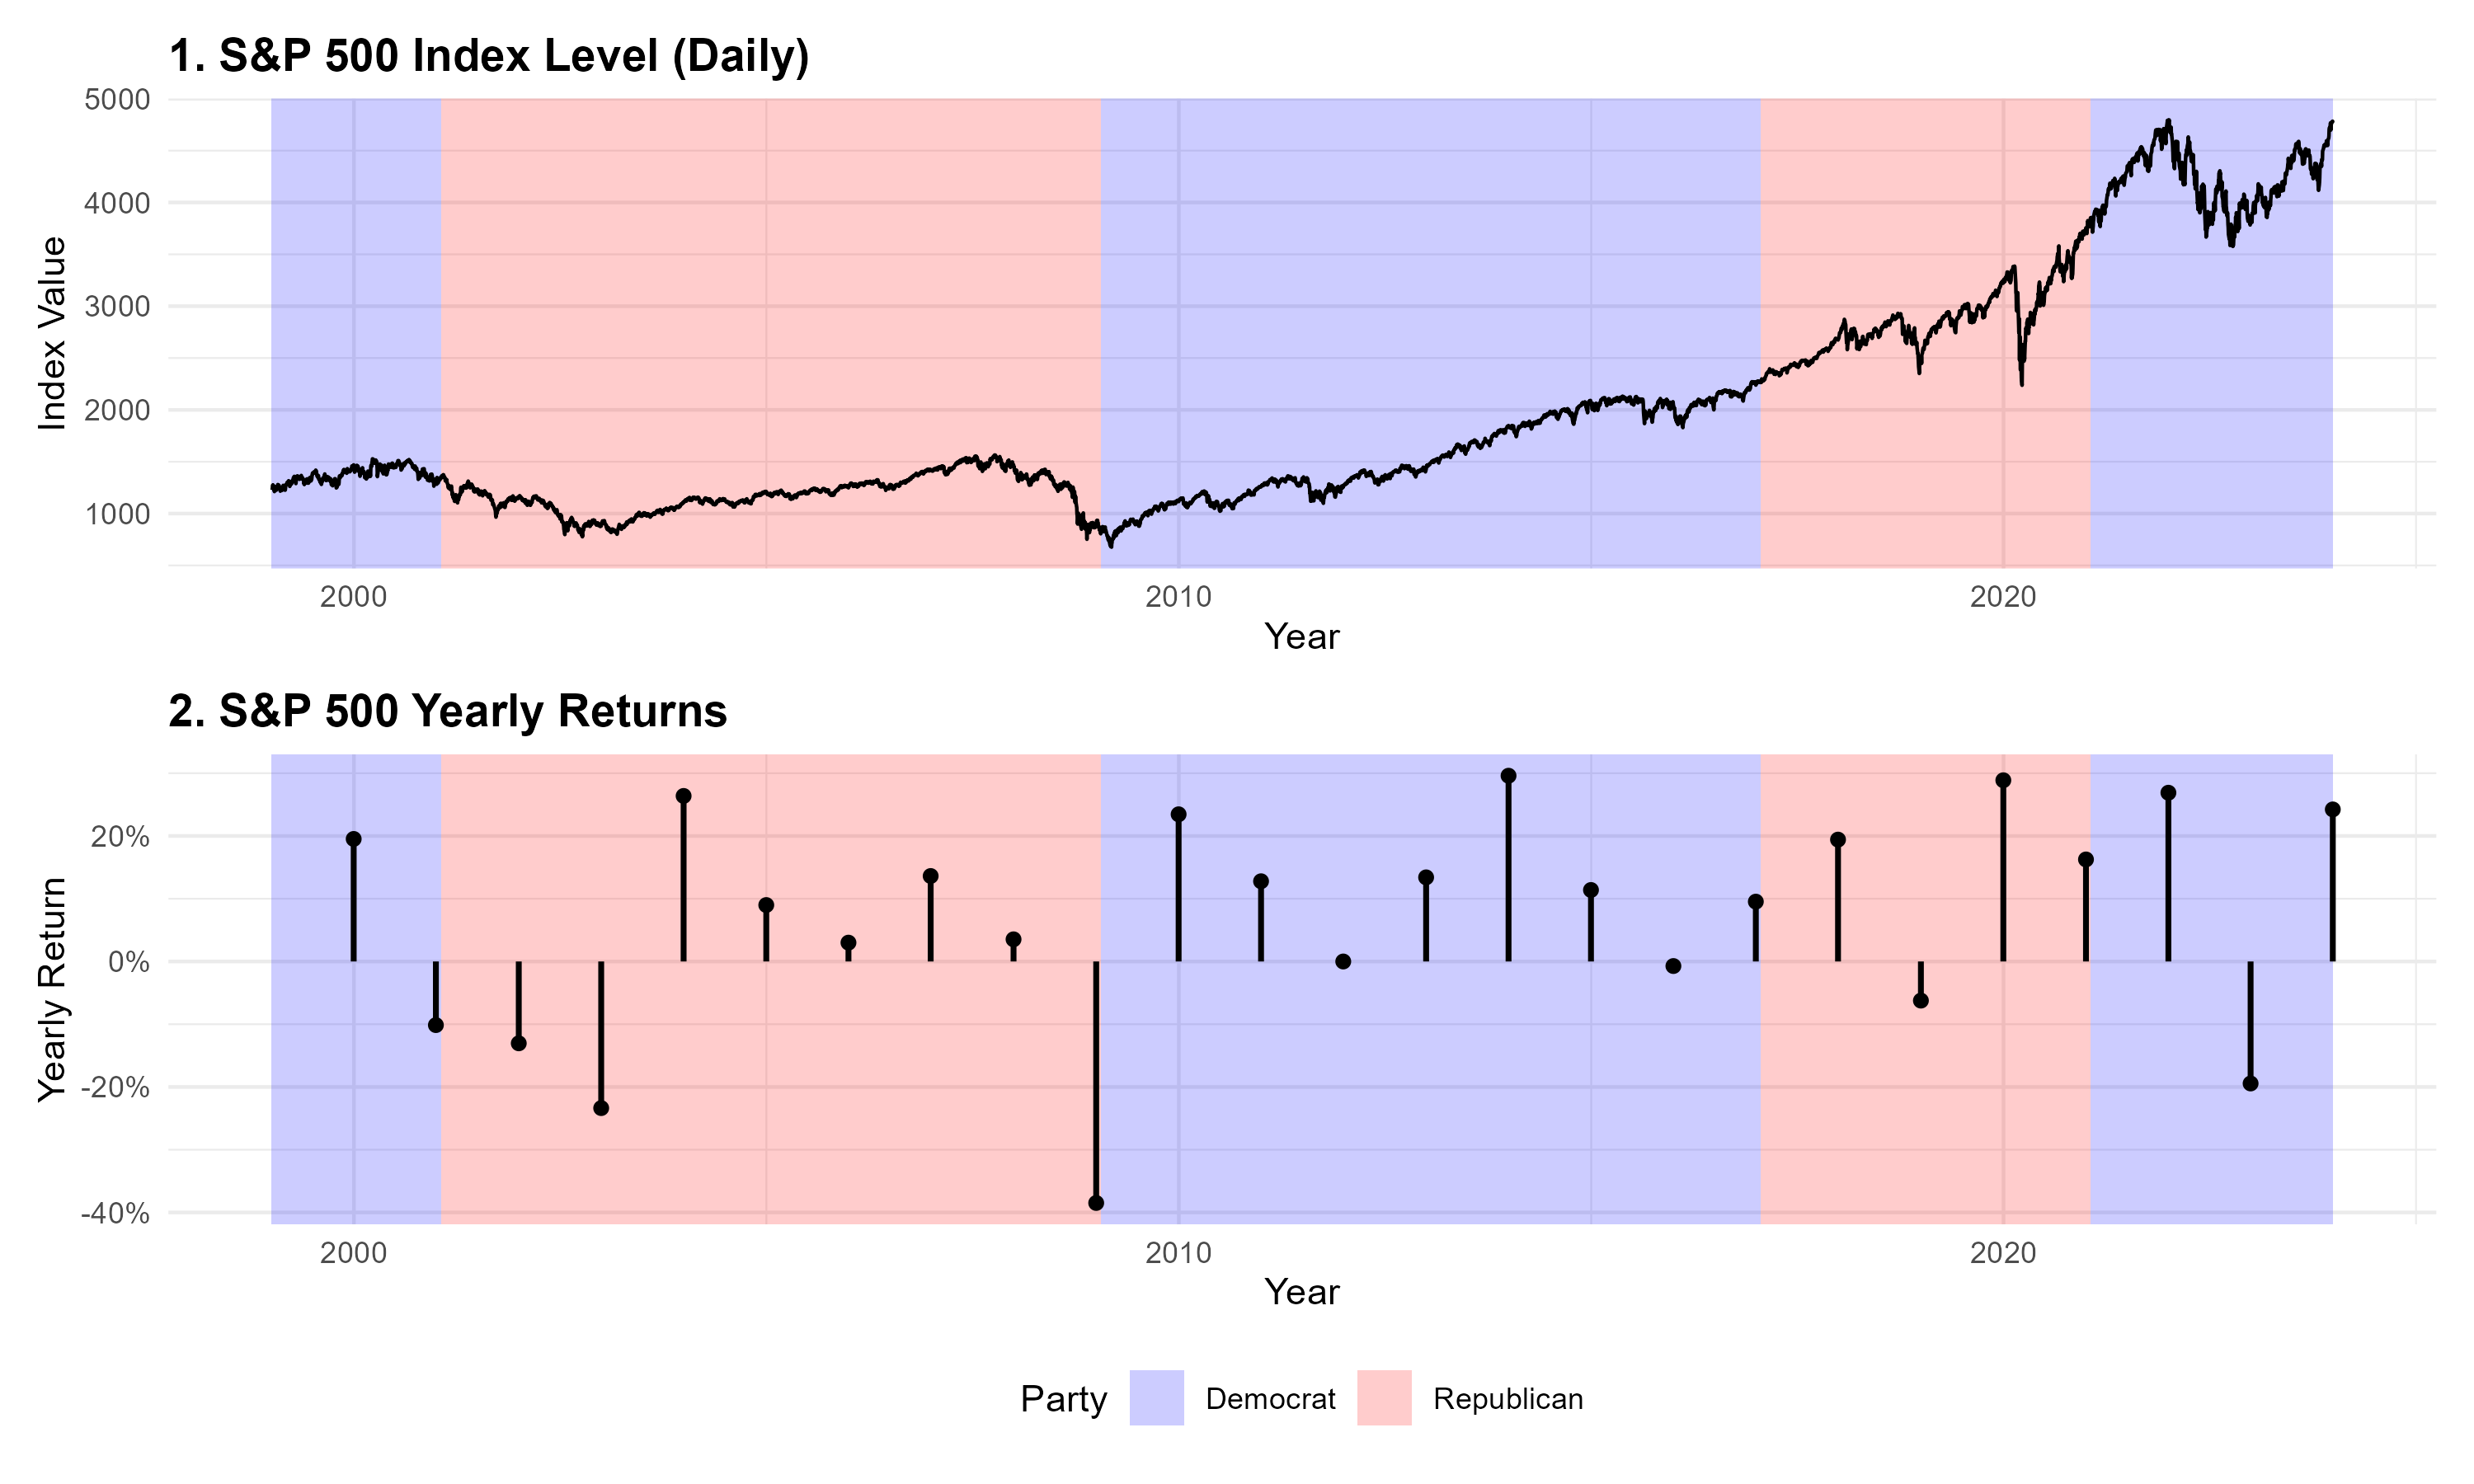
\includegraphics[width=\textwidth]{./figures/sp500.png}
    
    \begin{minipage}{\textwidth}
        \footnotesize This figure illustrates the historical performance of the S\&P 500 index throughout the sample period 1999-2023, overlaid with the corresponding U.S. presidential administrations. The top panel shows the the daily closing index value. The bottom panel marks the annual returns at the year-end. For example, the return plotted at 2000 represents the return from the end of 1999 to the end of 2000. The vertical background shading serves as a visual timeline for the federal political environment. Light blue shading designates periods during which the presidency was held by a Democrat, while the light red shading designates periods during which the presidency was held by a Republican.
    \end{minipage}
\end{figure}



\Cref{fig:sp500} illustrates the performance of the S\&P 500 index throughout the sample period, overlaid with the corresponding U.S. presidential administrations. The vertical background shading serves as a visual timeline for the federal political environment. The sample period encompasses both the dot-com bubble collapse and the Global Financial Crisis (GFC), both of which occurred during a Republican presidency. As illustrated by the S\&P 500 Yearly Returns chart, these periods are marked by severe negative market contractions, including a near -40\% yearly return drop in 2008, perfectly overlapping with the Republican-shaded timeline.

Conversely, the subsequent post-GFC bull market occurred during a Democratic presidency. The daily S\&P 500 index level shows a steady, prolonged upward trajectory during this Democrat-shaded period from roughly 2009 to 2017, accompanied by consistently positive yearly returns. Because these severe macroeconomic shocks and subsequent recoveries correlate so strongly with the alternating federal administrations in this specific timeframe, the FEDIR variable likely captures the mechanical suppression of stock market participation caused by these broader economic crises rather than a direct political effect.

Ultimately, this initial glance at the alignment data can be misleading if interpreted as a behavioral shift. As established in the direction reconciliation analysis, the aggregated state alignment variable is not a direct proxy for individual political preferences. Therefore, the lack of a significant state-level alignment effect is not a contradictory result to established literature, but rather a reflection of macroeconomic time-series variation and the limitations of ecological aggregation.



% !TEX root = ../main.tex

\section{Channels}
\label{sec:channels}

In reconciling the aggregate state-level findings with the individual-level literature, an open discussion remains as to specifically how the political divide affects the baseline differences in SMP rate. 'Red' and 'blue' states could be viewed not merely as political labels, but as proxies representing the true instrument that impact the financial behavior of residents.

Any plausible channel must satisfy three specific criteria based on the empirical results. First, it must support higher baseline SMP in 'blue' states than in 'red' states. Second, it must represent a structural state-level difference or an unobserved individual heterogeneity not captured by standard demographic controls. Third, it must exclusively affect the probability of participation without influencing the conditional equity share among participants, likely by affecting a one-time fixed cost of entry rather than risk preferences. 

Several structural state-level differences could serve as the underlying mechanism for this gap. The suggestions below are merely speculative and empirical tests would require additional data and analysis that are beyond the scope of this paper.

\vspace{2em}

\noindent\textbf{Industry Composition:}\\[0.5em]
One possibility is the geographic distribution of publicly listed firms. Geographic proximity to a firm can increase the likelihood of local residents investing in that firm as proximity facilitates easier access to information and lowers monitoring costs. For example, \citet{coval2001} finds that fund managers perform better when investing in nearby firms. 

\noindent If 'blue' states systematically house a higher concentration of publicly traded companies and corporate headquarters, this would create state-level differences in the fixed information costs required to invest, with residents in 'blue' states facing lower baseline hurdles to participation. This framework assumes that stock market participation is a combination of individual decisions to invest in independent firms rather than a broad participate-then-allocate decision.

\vspace{1em}
\noindent\textbf{Local Culture and Peer Effects:}\\[0.5em]
Following the literature on social interactions (e.g., \citet{hong2004}), state-level variations in social dynamics could play a significant role. If the cultural environment in Democratic states fosters social networks that more efficiently share investment information (e.g. whether it is deemed a cultural taboo to discuss money), this could lead to higher participation through an information cost channel. Alternatively, this could operate through a trust channel: lower trust in the financial system has been shown to be associated with lower propensity to participate \citep{guiso2008, giannetti2016, bu2022, huang2023}. If baseline trust or distrust in financial markets is circulated via local socializing or historical experiences re-circulated among residents, this could create state-level differences in the fixed costs of entering the market. Both variations help overcome the initial hurdle of entering the market, but do not necessarily affect the risk preferences of those who have already decided to participate.

\vspace{1em}
\noindent\textbf{Binding Liquidity Constraints (Urban vs. Rural):}\\[0.5em]
The urban-rural divide is a well-documented phenomenon in the political science literature \citep{rodden2019cities, gimpel2020}. Urban centers, overwhelmingly located in Democratic-leaning states, generally feature significantly higher costs of living, particularly rent prices. Consequently, individuals are often liquidity-constrained and unable to accumulate the massive down payments required for homeownership or small business ventures. Instead of tying up wealth in illiquid real estate, these individuals invest their available savings into liquid assets like the stock market. In contrast, residents in rural, Republican-leaning areas face lower living costs and looser liquidity constraints, allowing them to allocate capital into housing or local businesses. Under such a framework, binding liquidity constraints can act as a structural determinant of the fixed participation decision.

\vspace{1em}
\noindent\textbf{Financial Literacy and Cognitive Fixed Costs:}\\[0.5em]
While this paper controls for a binary college indicator, this fails to capture more complex variations in K-12 curricula or the dominant types of degrees earned across states. This can create differences in financial literacy that are not fully captured by standard demographic controls. \citet{vanrooij2011, bernheim2001, bernheim2003} among others have shown that improved financial literacry through education has a positive impact on stock market participation. Higher financial literacy equips individuals to navigate complex financial products, thereby directly reducing the cognitive fixed costs of entering the stock market and facilitating market participation. If residents in 'blue' states, either by growing up there and those states having better financial education, or by systematic migration of more financially literate individuals, are more likely to be more financially literate, this could drive the observed differences in baseline SMP rates and vice versa.

\vspace{2em}

In reality, the observed baseline differences in stock market participation are likely driven by a complex mixture of these structural, cultural, and economic factors. Pinpointing the exact causal mechanism through which specific state environments influence market entry is an exceedingly complicated question that is difficult to answer definitively with the observational data at hand, and thus remains an open question for future research.

Ultimately, the primary contribution of this paper is not in isolating a single, definitive channel. Rather, the contribution lies in successfully identifying that the state differences creating the gap in baseline participation rates are in the opposite direction of the individual-level behavioral preferences and that the gap is robustly correlated with the partisan divide. By disentangling the aggregate structural mechanisms from individual-level behavioral preferences, this paper provides a clearer framework for understanding the macroeconomic implications of political geography on financial markets.

% !TEX root = ../main.tex

\section{Conclusion}

This study investigates the persistent geographic (state-level) differences in U.S. stock market participation (SMP) rates, a phenomenon that standard demographic and financial characteristics cannot fully explain. Utilizing household-level panel data from the PSID spanning 1999 to 2023, paired with state-level political orientation metrics derived from FEC campaign contributions, the analysis tests whether the political environment of a state acts as a structural driver of financial behavior. The empirical tests evaluate both the initial decision (STOCKHOLD) and the allocation conditional on participation (STOCKSHARE). The most important finding is the presence of a Simpson's paradox: while individual-level shifts toward Republican preferences increase the likelihood of investing, aggregate baseline participation rates are systematically higher in Democratic-leaning states. This state-level political influence acts exclusively on the initial fixed-cost hurdle of entering the market, without affecting the conditional equity share given participation. 

By disentangling these effects, this paper contributes to the literature by bridging the gap between individual-level behavioral finance and state-level political geography to explain the persistent geographic variations in U.S. stock market participation. While a shift toward Republican preferences increases an individual's likelihood of investing,  aggregate baseline participation rates are systematically higher in Democratic-leaning states, and this state-level difference dominates. Notably, this state-level political influence acts exclusively on the initial fixed-cost hurdle of entering the market, without affecting the conditional equity share given participation. 

A major limitation of this paper is that the specific underlying mechanism or channel is yet unclear. Potential channels include corporate industry concentration, urban liquidity constraints forcing liquid investments, or cultural differences in financial literacy and information-sharing, etc., but these remain as speculative conjectures that require further causal investigation. Future research could empirically test these channels by merging additional state-level data on properties such as urbanization, industry concentration, education policies, etc. 

Another limitation is that the state-federal alignment measure's impact may have been underestimated in this methodology. The stock holdings data from PSID is biennial whereas political variables are updated every four years. Furthermore, the sample period saw frequent midterm election reversals, suggesting that alignment may have weakened or strengthened on a more short-term basis. This could have potentially diluted the alignment effects and led to the insignificant findings. However, extending the interpretation from absolute directional analysis that state politics reflect structural differences rather than proxies for individual preferences, this sounds unlikely. 

% --- Bibliography ---
% exported from Zotero with Better BibTeX
\newpage
\printbibliography

% --- Appendices ---
\newpage
\begin{appendices}
\crefalias{section}{appendix}
\counterwithin{table}{section}
\counterwithin{figure}{section}
% !TEX root = ../main.tex

\section{Construction of PSID Variables}
\label{sec:appendix_psid}

This section describes in detail how the varaibles from the PSID dataset were constructed. The underlying data is sourced from the Panel Study of Income Dynamics (PSID) Family-Level files, spanning the biennial survey waves from 1999 to 2023 (odd years).The equations below formally define how the final analytical variables are mapped and calculated directly as a function of the raw, reshaped PSID base variables. \Cref{tab:A1} details the specific variable codes across all waves used to construct the base variables.

$$
\begin{aligned}
\text{stockhold} &= \mathbf{1}(\text{wthstckimptf} = 1) \\[8pt]
\text{finassets} &= 
\begin{cases} 
\text{wthcashbondimpval} + \text{wthstckimpval}, & ( t \le 2017 ) \\
\text{wthcashimpval} + \text{wthbondimpval} + \text{wthstckimpval}, & ( t \ge 2019 ) 
\end{cases} \\[8pt]
\text{stockshare} &= \min \left( \frac{\text{wthstckimpval}}{\text{finassets}}, 1 \right) \quad \text{for finassets} > 0 \\[8pt]
\text{stockhold\_ira} &= \mathbf{1}(\text{retirementalloc} \in \{1, 3\}) \\[8pt]
\text{stockhold\_pen} &= \mathbf{1}(\text{pensionallochd} \in \{1, 2\} \lor \text{pensionallocsp} \in \{1, 2\}) \\[8pt]
\text{stockhold\_tot} &= \mathbf{1}(\text{stockhold} = 1 \lor \text{stockhold\_ira} = 1 \lor \text{stockhold\_pen} = 1) \\[8pt]
\text{lnincome} &= \ln(\text{incfamilytotal}) \quad \text{for incfamilytotal} > 0 \\[8pt]
\text{lnwealth} &= \ln(\text{wthtotinclheq}) \quad \text{for wthtotinclheq} > 0 \\[8pt]
\text{college} &= \mathbf{1}(\text{eduhdcoldegtf} = 1) \\[8pt]
\text{age} &= \text{agehd} \quad \text{for agehd} \neq 999 \\[8pt]
\text{male} &= \mathbf{1}(\text{sexhd} = 1)
\end{aligned}
$$

\begin{sidewaystable}[htbp]
    \centering
    \caption{PSID Wave-Specific Variable Codes}
    \label{tab:A1}
    \footnotesize
    
    \begin{tabularx}{\textheight}{@{} l l X c X @{}}
    \toprule
    \textbf{Final Variable} & \textbf{Base Variable} & \textbf{Definition \& Construction} & \textbf{Years} & \textbf{Variable Codes (from old to recent)} \\
    \midrule
    
    \textbf{\texttt{stockhold}} & \texttt{wthstckimptf} & Binary indicator for direct stock ownership. Set to 1 if \texttt{wthstckimptf} == 1. & 1999--2023 & S410 S510 S610 S710 S810 ER46952 ER52356 ER58169 ER65366 ER71443 ER77469 ER81796 ER85650 \\
    \addlinespace
    
    \textbf{\texttt{stockshare}} & \texttt{wthstckimpval} & Numerator for stock share calculation. & 1999--2023 & S411 S511 S611 S711 S811 ER46954 ER52358 ER58171 ER65368 ER71445 ER77471 ER81798 ER85652 \\
    \addlinespace
    
     & \texttt{wthcashbondimpval} & Denominator component for financial assets (1999-2017). & 1999--2017 & S405 S505 S605 S705 S805 ER46942 ER52350 ER58161 ER65358 ER71435 \\
    \addlinespace
    
     & \texttt{wthcashimpval} & Denominator cash component for financial assets (2019-2023). & 2019--2023 & ER77457 ER81784 ER85638 \\
    \addlinespace
    
    & \texttt{wthbondimpval} & Denominator bond component for financial assets (2019-2023). & 2019--2023 & ER77461 ER81788 ER85642 \\
    \addlinespace
    
    \textbf{\texttt{stockhold\_tot}} & \texttt{retirementalloc} & IRA/Annuity component for broad stockholding indicator. & 1999--2023 & ER15013 ER19209 ER22589 ER26570 ER37588 ER43579 ER48904 ER54654 ER61765 ER67818 ER73841 ER79963 ER83932 \\
    \addlinespace
    
     & \texttt{pensionallochd} & Head pension component for broad stockholding indicator. & 1999--2023 & ER15182 ER19350 ER22745 ER26726 ER37766 ER43739 ER49085 ER54841 ER61961 ER68015 ER74041 ER80164 ER84134 \\
    \addlinespace
    
     & \texttt{pensionallocsp} & Spouse pension component for broad stockholding indicator. & 1999--2023 & ER15328 ER19493 ER22889 ER26870 ER37998 ER43971 ER49304 ER55057 ER62178 ER68232 ER74248 ER80370 ER84340 \\

    \bottomrule
    \end{tabularx}
\end{sidewaystable}

\begin{sidewaystable}[htbp]
    \centering
    \ContinuedFloat
    \caption[]{PSID Wave-Specific Variable Codes (Cont.)}
    \footnotesize
    
    \begin{tabularx}{\textheight}{@{} l l X c X @{}}
    \toprule
    \textbf{Final Variable} & \textbf{Base Variable} & \textbf{Definition \& Construction} & \textbf{Years} & \textbf{Variable Codes (from old to recent)} \\
    \midrule
    
    \textbf{\texttt{lnincome}} & \texttt{incfamilytotal} & Natural log of total family income. & 1999--2023 & ER16462 ER20456 ER24099 ER28037 ER41027 ER46935 ER52343 ER58152 ER65349 ER71426 ER77448 ER81775 ER85629 \\
    \addlinespace
    
    \textbf{\texttt{lnwealth}} & \texttt{wthtotinclheq} & Natural log of total family wealth. & 1999--2023 & S417 S517 S617 S717 S817 ER46970 ER52394 ER58211 ER65408 ER71485 ER77511 ER81838 ER85692 \\
    \addlinespace
    
    \textbf{\texttt{college}} & \texttt{eduhdcoldegtf} & Binary indicator for household head possessing a college degree. & 1999--2023 & ER15952 ER20013 ER23450 ER27417 ER40589 ER46567 ER51928 ER57684 ER64836 ER70908 ER76923 ER81170 ER85147 \\
    \addlinespace
    
    \textbf{\texttt{age}} & \texttt{agehd} & Age of Household Head (excluding missing values coded as 999). & 1999--2023 & ER13010 ER17013 ER21017 ER25017 ER36017 ER42017 ER47317 ER53017 ER60017 ER66017 ER72017 ER78017 ER82018 \\
    \addlinespace
    
    \textbf{\texttt{male}} & \texttt{sexhd} & Binary indicator for male household head (set to 1 if \texttt{sexhd} == 1). & 1999--2023 & ER13011 ER17014 ER21018 ER25018 ER36018 ER42018 ER47318 ER53018 ER60018 ER66018 ER72018 ER78018 ER82019 \\
    \addlinespace
    
    \textbf{\texttt{state}} & \texttt{currfips} & US State FIPS Code (values 1 through 56). & 1999--2023 & ER13005 ER17005 ER21004 ER25004 ER36004 ER42004 ER47304 ER53004 ER60004 ER66004 ER72004 ER78004 ER82004 \\
    \addlinespace
    
    \textbf{\texttt{seqnum}} & \texttt{seqnumY} & Filtering variable to isolate Household Heads (\texttt{seqnum} == 1). & 1999--2023 & ER33502 ER33602 ER33702 ER33802 ER33902 ER34002 ER34102 ER34202 ER34302 ER34502 ER34702 ER34902 ER35102 \\
    \addlinespace
    
    \textbf{\texttt{currfamid}} & \texttt{idfam} & Current wave-specific family ID construction. & 1999--2023 & ER13002 ER17002 ER21002 ER25002 ER36002 ER42002 ER47302 ER53002 ER60002 ER66002 ER72002 ER78002 ER82002 \\
    \bottomrule
    \end{tabularx}
\end{sidewaystable}
% !TEX root = ../main.tex

\section{Construction of FEC Contribution Share Variables}
\label{sec:appendix_fecscreen}

This appendix provides a formal breakdown of the algorithm and filtering methodology used to construct the state-level political orientation metrics from the Federal Election Commission (FEC) campaign finance datasets. The screening framework eliminates intra-party conflict, non-individual contributions, conduit noise, and issue-based Political Action Committees (PACs) to accurately extract grassroots partisan leaning across presidential election years (1996, 2000, 2004, 2008, 2012, 2016, 2020).

\subsection{Candidate Filtering and Identification}
To isolate contributions that reflect general election partisan alignment, the candidate master universe is first restricted to the two major parties: Democrats (\texttt{DEM}) and Republicans (\texttt{REP}). For presidential cycles, inclusion is strictly limited to the ultimate primary winners who advanced to the general election, following \citet{meeuwis2022}. This prevents heightend intra-party competition (e.g., primary campaigns) from inflating a state's partisan polarization index. Voters supporting a losing primary candidate do not necessary support the general election nominee, and thus their contributions are not indicative of the state's overall partisan leaning in the general election.

Let $\mathcal{C}_t$ denote the set of valid presidential candidates in election cycle $t$:
\begin{align*}
    \mathcal{C}_{1996} &= \{\text{Bill Clinton (DEM)}, \text{Bob Dole (REP)}\} \\
    \mathcal{C}_{2000} &= \{\text{Al Gore (DEM)}, \text{George W. Bush (REP)}\} \\
    \mathcal{C}_{2004} &= \{\text{John Kerry (DEM)}, \text{George W. Bush (REP)}\} \\
    \mathcal{C}_{2008} &= \{\text{Barack Obama (DEM)}, \text{John McCain (REP)}\} \\
    \mathcal{C}_{2012} &= \{\text{Barack Obama (DEM)}, \text{Mitt Romney (REP)}\} \\
    \mathcal{C}_{2016} &= \{\text{Hillary Clinton (DEM)}, \text{Donald Trump (REP)}\} \\
    \mathcal{C}_{2020} &= \{\text{Joe Biden (DEM)}, \text{Donald Trump (REP)}\}
\end{align*}

\subsection{Multi-Stage Committee Screening Algorithm}
Committees ($c$) are classified into one of four categories: Democratic (\texttt{DEM}), Republican (\texttt{REP}), Excluded (\texttt{EXC}), or Indeterminate (\texttt{IND}). Classification follows a four-step sequence:

\subsubsection{Stage 1: Institutional Code Classification}
Initial filtering relies on the FEC committee type designations (\texttt{cmte\_tp}):
\begin{itemize}
    \item \texttt{EXC}: Communication costs (\texttt{C}), presidential primaries (\texttt{D}), electioneering communications (\texttt{E}), house committees (\texttt{H}), independent expenditors (\texttt{I}), and senate committees (\texttt{S}) are definitively removed.
    \item Committees categorized as party organizations (\texttt{X}, \texttt{Y}, \texttt{Z}) are automatically mapped to \texttt{DEM} or \texttt{REP} matching their reported party affiliation (\texttt{cmte\_pty\_affiliation}). If they report any other party affiliation, they are marked \texttt{EXC}.
    \item Standard PACs (\texttt{N}, \texttt{Q}), Super PACs (\texttt{O}), Hybrid PACs (\texttt{V}, \texttt{W}), single-candidate independent entities (\texttt{U}), and core presidential committees (\texttt{P}) are set as \texttt{IND} and sent to the next stage.
\end{itemize}

\subsubsection{Stage 2: Official Candidate Linkage}
For any committee still marked \texttt{IND}, if it possesses an official candidate link (\texttt{cand\_id}):
\begin{equation}
    \text{Status}(c) = \begin{cases} 
        \texttt{DEM} & \text{if } \texttt{cand\_id}_c \in \mathcal{C}_t \text{ and Party}(\texttt{cand\_id}_c) = \texttt{DEM} \\
        \texttt{REP} & \text{if } \texttt{cand\_id}_c \in \mathcal{C}_t \text{ and Party}(\texttt{cand\_id}_c) = \texttt{REP} \\
        \texttt{EXC} & \text{if } \texttt{cand\_id}_c \notin \mathcal{C}_t \text{ and } \texttt{cand\_id}_c \neq \emptyset \\
        \texttt{IND} & \text{otherwise} \\
    \end{cases}
\end{equation}

\subsubsection{Stage 3: Unofficial Linkage via Independent Expenditures}
For unlinked PACs, behavior is inferred using individual transaction data from the independent expenditure files (\texttt{pas2}). Valid expenditures supporting or opposing candidates are quantified. Let $N_{\text{for}, p}$ and $A_{\text{for}, p}$ represent the total transaction count and aggregate dollar volume spent \textit{supporting} party $p \in \{\text{DEM}, \text{REP}\}$, and let $N_{\text{agt}, p}$ and $A_{\text{agt}, p}$ represent expenditure amounts spent \textit{opposing} party $p$. 

We construct committee-level two directional indexes normalized to $[-1, 1]$, where $+1$ represents purely Republican support and $-1$ represents purely Democratic support:
\begin{equation}
    \mathcal{I}_{n}(c) = 2 \times \left( \frac{N_{\text{for, REP}} + N_{\text{agt, DEM}}}{N_{\text{total}}} \right) - 1
\end{equation}
\begin{equation}
    \mathcal{I}_{\text{sum}}(c) = 2 \times \left( \frac{A_{\text{for, REP}} + A_{\text{agt, DEM}}}{A_{\text{total}}} \right) - 1
\end{equation}
Committees with extreme, uniform alignment are captured as partisan vehicles:
\begin{equation}
    \text{Status}(c) = \begin{cases} 
        \texttt{DEM} & \text{if } \mathcal{I}_{n}(c) \le -0.75 \text{ and } \mathcal{I}_{\text{sum}}(c) \le -0.75 \\
        \texttt{REP} & \text{if } \mathcal{I}_{n}(c) \ge 0.75 \text{ and } \mathcal{I}_{\text{sum}}(c) \ge 0.75 
    \end{cases}
\end{equation}

\subsubsection{Stage 4: Text-Pattern Regex Targeted Capture}
Remaining \texttt{IND} committees are passed through a case-insensitive regular expression keyword check targeting party infrastructure and candidate names:
\begin{itemize}
    \item {Democratic Keywords}: Candidate last names in $\mathcal{C}_{t,\text{DEM}}$, \texttt{DNC}, \texttt{DSCC}, \texttt{DCCC}, \texttt{DEMOCRATIC}, \texttt{DEMOCRAT(S)}, \texttt{SENATE MAJORITY PAC}, \texttt{HOUSE MAJORITY PAC}.
    \item {Republican Keywords}: Candidate last names in $\mathcal{C}_{t,\text{REP}}$, \texttt{RNC}, \texttt{NRSC}, \texttt{NRCC}, \texttt{GOP}, \texttt{REPUBLICAN(S)}, \texttt{CONGRESSIONAL LEADERSHIP FUND}, \texttt{SENATE LEADERSHIP FUND}.
\end{itemize}

\subsubsection{Stage 5: Secondary Manual Screening and Overrides}
To guarantee that the selected active portfolio isolates core partisan alignment without introducing non-comparable baseline noise, a targeted manual screening is applied to high-volume committees:
\begin{itemize}
    \item Automated intermediary fundraising platforms (e.g., \texttt{ACTBLUE}) are explicitly set to \texttt{EXC} to eliminate baseline inflation, as individual allocations are already captured downstream at their final committee destinations.
    \item Ideological PACs that frequently back internal party primary candidates or prioritize single-issue advocacy (e.g., \texttt{EMILY'S LIST}, \texttt{FAIR FIGHT}, \texttt{AMERICANS FOR PROSPERITY ACTION}, \texttt{CLUB FOR GROWTH ACTION}) are systematically marked \texttt{EXC}.
    \item Industry-specific lobbying coalitions and profession-based bodies (e.g., automotive dealers, realtors, law associations, or corporate consulting PACs) are marked \texttt{EXC}..
    \item Specialized party or candidate-adjacent Super PACs with atypical names (e.g., \texttt{COMMITTEE FOR CHANGE}, \texttt{SMP}, \texttt{TAKE BACK THE HOUSE 2020}) are manually preserved as \texttt{DEM} or \texttt{REP} following manual verification.
\end{itemize}

\subsubsection{Final Set of committees}
\Cref{tab:B1} lists ten of the finally selected committees for each year, ordered by the number of total valid contributions. 

\begin{table}[tbp] \centering
\newcolumntype{R}{>{\raggedleft\arraybackslash}X}
\newcolumntype{L}{>{\raggedright\arraybackslash}X}
\newcolumntype{C}{>{\centering\arraybackslash}X}

\caption{Top 10 Selected Committees by Election Year}
\label{tab:B1}

\footnotesize
\begin{tabularx}{\linewidth}{c L c r r}

\toprule
{Year}&{Committee Name}&{Party}&{N}&{Amount} \tabularnewline
\midrule \addlinespace[\belowrulesep]
1996&REPUBLICAN NATIONAL COMMITTEE - RNC&REP&61957&39243617 \tabularnewline
&NATIONAL REPUBLICAN CONGRESSIONAL COMMITTEE CONTRIBUTIONS&REP&55651&21067394 \tabularnewline
&DOLE FOR PRESIDENT INC&REP&32673&19303022 \tabularnewline
&CLINTON/GORE '96 PRIMARY COMMITTEE INC&DEM&27579&18678797 \tabularnewline
&DNC SERVICES CORPORATION/DEMOCRATIC NATIONAL COMMITTEE&DEM&26444&33411231 \tabularnewline
&NATIONAL REPUBLICAN SENATORIAL COMMITTEE&REP&26074&17532726 \tabularnewline
&DEMOCRATIC SENATORIAL CAMPAIGN COMMITTEE&DEM&4801&10665441 \tabularnewline
&DEMOCRATIC CONGRESSIONAL CAMPAIGN COMMITTEE&DEM&4258&5527039 \tabularnewline
&CLINTON/GORE '96 GEN ELECTION LEGAL \& ACCOUNTING COMPLIANCE&DEM&3643&1926508 \tabularnewline
&DOLE/KEMP '96 COMPLIANCE COMMITTEE INC&REP&3403&2280408 \tabularnewline
2000&BUSH FOR PRESIDENT INC&REP&108472&73718740 \tabularnewline
&REPUBLICAN NATIONAL COMMITTEE - RNC&REP&91994&81798829 \tabularnewline
&NATIONAL REPUBLICAN CONGRESSIONAL COMMITTEE CONTRIBUTIONS&REP&59920&26023012 \tabularnewline
&DNC SERVICES CORPORATION/DEMOCRATIC NATIONAL COMMITTEE&DEM&46366&65189909 \tabularnewline
&GORE 2000 INC&DEM&41427&25422001 \tabularnewline
&NATIONAL REPUBLICAN SENATORIAL COMMITTEE&REP&15283&14461198 \tabularnewline
&GORE/LIEBERMAN GENERAL ELECTION LEGAL AND ACCOUNTING COMPLIANCE FUND&DEM&10384&6410557 \tabularnewline
&BUSH-CHENEY 2000 COMPLIANCE COMMITTEE INC&REP&9539&6770135 \tabularnewline
&DEMOCRATIC CONGRESSIONAL CAMPAIGN COMMITTEE-CONTRIBUTIONS&DEM&6138&8887916 \tabularnewline
&DEMOCRATIC SENATORIAL CAMPAIGN COMMITTEE&DEM&5171&9186161 \tabularnewline
2004&BUSH-CHENEY '04 INC&REP&196987&172686923 \tabularnewline
&JOHN KERRY FOR PRESIDENT, INC&DEM&193913&134195108 \tabularnewline
&REPUBLICAN NATIONAL COMMITTEE&REP&154445&166848971 \tabularnewline
&NATIONAL REPUBLICAN CONGRESSIONAL COMMITTEE&REP&151520&85608871 \tabularnewline
&DNC SERVICES CORPORATION/DEMOCRATIC NATIONAL COMMITTEE&DEM&148660&111769319 \tabularnewline
&KERRY VICTORY 2004&DEM&18892&39900592 \tabularnewline
&MOVEON PAC&DEM&18086&8541254 \tabularnewline
&BUSH-CHENEY '04 COMPLIANCE COMMITTEE INC.&REP&15733&13248329 \tabularnewline
&DEMOCRATIC CONGRESSIONAL CAMPAIGN COMMITTEE&DEM&14445&22942485 \tabularnewline
&KERRY-EDWARDS 2004 INC. GENERAL ELECTION LEGAL AND ACCOUNTING COMPLIANCE FUND&DEM&9449&7849447 \tabularnewline
\bottomrule

\end{tabularx}
\end{table}


\begin{table}[tbp] \centering
\newcolumntype{R}{>{\raggedleft\arraybackslash}X}
\newcolumntype{L}{>{\raggedright\arraybackslash}X}
\newcolumntype{C}{>{\centering\arraybackslash}X}

\ContinuedFloat
\caption[]{Top 10 Selected Committees by Election Year}
\footnotesize
\begin{tabularx}{\linewidth}{c L c r r}

\toprule
{Year}&{Committee Name}&{Party}&{N}&{Amount} \tabularnewline
\midrule \addlinespace[\belowrulesep]
2008&OBAMA FOR AMERICA&DEM&586385&305375905 \tabularnewline
&JOHN MCCAIN 2008 INC.&REP&192852&113007118 \tabularnewline
&REPUBLICAN NATIONAL COMMITTEE&REP&153308&102676723 \tabularnewline
&OBAMA VICTORY FUND&DEM&100727&173782157 \tabularnewline
&MCCAIN-PALIN VICTORY 2008&REP&71786&70354810 \tabularnewline
&NATIONAL REPUBLICAN CONGRESSIONAL COMMITTEE&REP&52022&38212496 \tabularnewline
&DNC SERVICES CORPORATION/DEMOCRATIC NATIONAL COMMITTEE&DEM&47724&43075410 \tabularnewline
&DEMOCRATIC SENATORIAL CAMPAIGN COMMITTEE&DEM&37653&75656317 \tabularnewline
&DEMOCRATIC CONGRESSIONAL CAMPAIGN COMMITTEE&DEM&26887&54122643 \tabularnewline
&NATIONAL REPUBLICAN SENATORIAL COMMITTEE&REP&24163&36781517 \tabularnewline
2012&OBAMA FOR AMERICA&DEM&432226&183162544 \tabularnewline
&ROMNEY FOR PRESIDENT INC.&REP&267105&198944084 \tabularnewline
&OBAMA VICTORY FUND 2012&DEM&199143&337726844 \tabularnewline
&ROMNEY VICTORY INC&REP&153000&427082486 \tabularnewline
&REPUBLICAN NATIONAL COMMITTEE&REP&103368&86067409 \tabularnewline
&DNC SERVICES CORPORATION/DEMOCRATIC NATIONAL COMMITTEE&DEM&47526&32684490 \tabularnewline
&DEMOCRATIC SENATORIAL CAMPAIGN COMMITTEE&DEM&39725&37229191 \tabularnewline
&DEMOCRATIC CONGRESSIONAL CAMPAIGN COMMITTEE&DEM&37588&36622429 \tabularnewline
&NATIONAL REPUBLICAN SENATORIAL COMMITTEE&REP&25625&47530495 \tabularnewline
&NATIONAL REPUBLICAN CONGRESSIONAL COMMITTEE&REP&20237&28755779 \tabularnewline
2016&HILLARY FOR AMERICA&DEM&2470529&275513725 \tabularnewline
&HILLARY VICTORY FUND&DEM&433735&413959093 \tabularnewline
&DCCC&DEM&423193&43381803 \tabularnewline
&REPUBLICAN NATIONAL COMMITTEE&REP&273264&89257279 \tabularnewline
&TRUMP MAKE AMERICA GREAT AGAIN COMMITTEE&REP&245288&67271640 \tabularnewline
&DNC SERVICES CORP./DEM. NAT'L COMMITTEE&DEM&243333&41360116 \tabularnewline
&DSCC&DEM&155483&50151683 \tabularnewline
&DONALD J. TRUMP FOR PRESIDENT, INC.&REP&148068&54199960 \tabularnewline
&NRSC&REP&107949&46881511 \tabularnewline
&MOVEON.ORG POLITICAL ACTION&DEM&62705&6762457 \tabularnewline
\bottomrule

\end{tabularx}
\end{table}


\begin{table}[tbp] \centering
\newcolumntype{R}{>{\raggedleft\arraybackslash}X}
\newcolumntype{L}{>{\raggedright\arraybackslash}X}
\newcolumntype{C}{>{\centering\arraybackslash}X}

\ContinuedFloat
\caption[]{Top 10 Selected Committees by Election Year (Cont.)}

\footnotesize
\begin{tabularx}{\linewidth}{c L c r r}

\toprule
{Year}&{Committee Name}&{Party}&{N}&{Amount} \tabularnewline
\midrule \addlinespace[\belowrulesep]
2020&REPUBLICAN NATIONAL COMMITTEE&REP&1749909&183523920 \tabularnewline
&TRUMP MAKE AMERICA GREAT AGAIN COMMITTEE&REP&1573965&251616570 \tabularnewline
&NRSC&REP&1438060&124814235 \tabularnewline
&WINRED&REP&1212898&-154593632 \tabularnewline
&DCCC&DEM&998346&70370581 \tabularnewline
&DONALD J. TRUMP FOR PRESIDENT, INC.&REP&826138&99219409 \tabularnewline
&DSCC&DEM&764756&128084912 \tabularnewline
&NRCC&REP&508154&49662605 \tabularnewline
&PROGRESSIVE TURNOUT PROJECT&DEM&470252&14016179 \tabularnewline
&BIDEN VICTORY FUND&DEM&428560&474896488 \tabularnewline
\bottomrule

\end{tabularx}
\end{table}


\subsection{Individual Contribution Level Processing}
Once the final set of partisan committees ($\mathcal{M}_{\text{DEM}, t}, \mathcal{M}_{\text{REP}, t}$) is confirmed, individual transactional receipts (\texttt{itcont}) are cleaned and processed according to strict data audit constraints:
\begin{enumerate}
    \item Only explicit, valid individual contribution and refund transaction types are retained (\texttt{10}, \texttt{11}, \texttt{15}, \texttt{15E}, \texttt{21Y}, \texttt{22Y}).
    \item Transactions that are clearly not individual (neither $\texttt{entity\_tp} = \texttt{"IND"}$ nor is missing). Transactions with an \texttt{other\_id} link are dropped to remove simple inter-organizational transfers.
    \item Contributions are filtered by geography to keep only donors with a verified residency code corresponding to the 50 US States or Washington, D.C..
    \item To properly measure total economic support, refund entries (\texttt{21Y}, \texttt{22Y}) are mathematically converted to negative absolute values before aggregation.
\end{enumerate}

\subsection{Aggregation and Variable Metrics}
Valid transactions are aggregated to the state level using the donor's reported state residency code ($s \in \{\text{50 US States}, \text{DC}\}$). For each state $s$ and election cycle $t$, metrics are calculated in two methods ($X$): Net Dollar Amount (\texttt{tot\_amt}, postivie contributions amount net of refunds) and Strictly Positive Contribution Count (\texttt{n\_trans\_pos}, only counting strictly positive contributions). 

The metric for the Republican share of contributions is defined as:
\begin{equation}
    \text{Share}_{X, s, t} = \frac{X_{\text{REP}, s, t}}{X_{\text{REP}, s, t} + X_{\text{DEM}, s, t}}
\end{equation}
To calculate the finalized political alignment variable ($\text{STDIR}_{X, s, t}$), the shares are scaled linearly to fall within the $[-1, 1]$ interval:
\begin{equation}
    \text{STDIR}_{X, s, t} = 2 \times \text{Share}_{X, s, t} - 1
\end{equation}
A final value of $+1$ indicates an entirely Republican contributing base and $-1$ represents an entirely Democratic base.
\end{appendices}

\end{document}